\documentclass[11pt,a4paper]{article}
\usepackage[utf8]{inputenc}
\usepackage[margin=1in]{geometry}
\usepackage{amsmath}
\usepackage{amssymb}
\usepackage{graphicx}
\usepackage{hyperref}
\usepackage{listings}
\usepackage{xcolor}
\usepackage{booktabs}
\usepackage{float}

% Python code styling
\lstset{
    language=Python,
    basicstyle=\ttfamily\small,
    keywordstyle=\color{blue},
    commentstyle=\color{gray},
    stringstyle=\color{red},
    showstringspaces=false,
    breaklines=true,
    frame=single,
    backgroundcolor=\color{gray!10}
}

\title{Machine Learning Assignment 3}
\author{Dataset IDs: \# id:22--44-22-1 and \# id:22--44--22-1}
\date{}

\begin{document}

\maketitle

\begin{center}
Name: Sayan Mondal\\
Student ID: 24377372\\
Strand: Future Networked Systems\\
Course: MSc. Computer Science
\end{center}
    
\vspace{1em}

\section*{(i) Dataset 1}

\subsection*{(a)}

I performed 5-fold cross-validation using F1 score as the performance metric to select hyperparameters jointly through grid search.

\subsubsection*{(i)}

\textbf{Methodology:} Tested polynomial degrees $q \in \{1, 2, 3, 4, 5\}$ with regularization parameter $C \in \{0.001, 0.01, 0.1, 1, 10, 100, 1000\}$ using \texttt{sklearn.preprocessing.PolynomialFeatures} to augment input features.

\textbf{Results:} 
Cross validation analysis (In Figure \ref{fig:dataset1_logistic_cv}) we can see that $q=1$ works best out of all $C$ values we have checked. Higher-order polynomials ($q>1$) always work similarly or worse, indicating that the data lacks learnable nonlinear structure.
The CV F1 scores are also similar at about 0.80 with or without polynomial complexity.

\textbf{Interpretation:} The showing of the preference for linear features ($q=1$) along with the similar F1 scores at different model complexities appears to suggest that the model is actually not learning discriminative decision boundaries but rather resorting to majority class prediction due to the lack of sufficient discriminative features.

\begin{figure}[H]
\centering
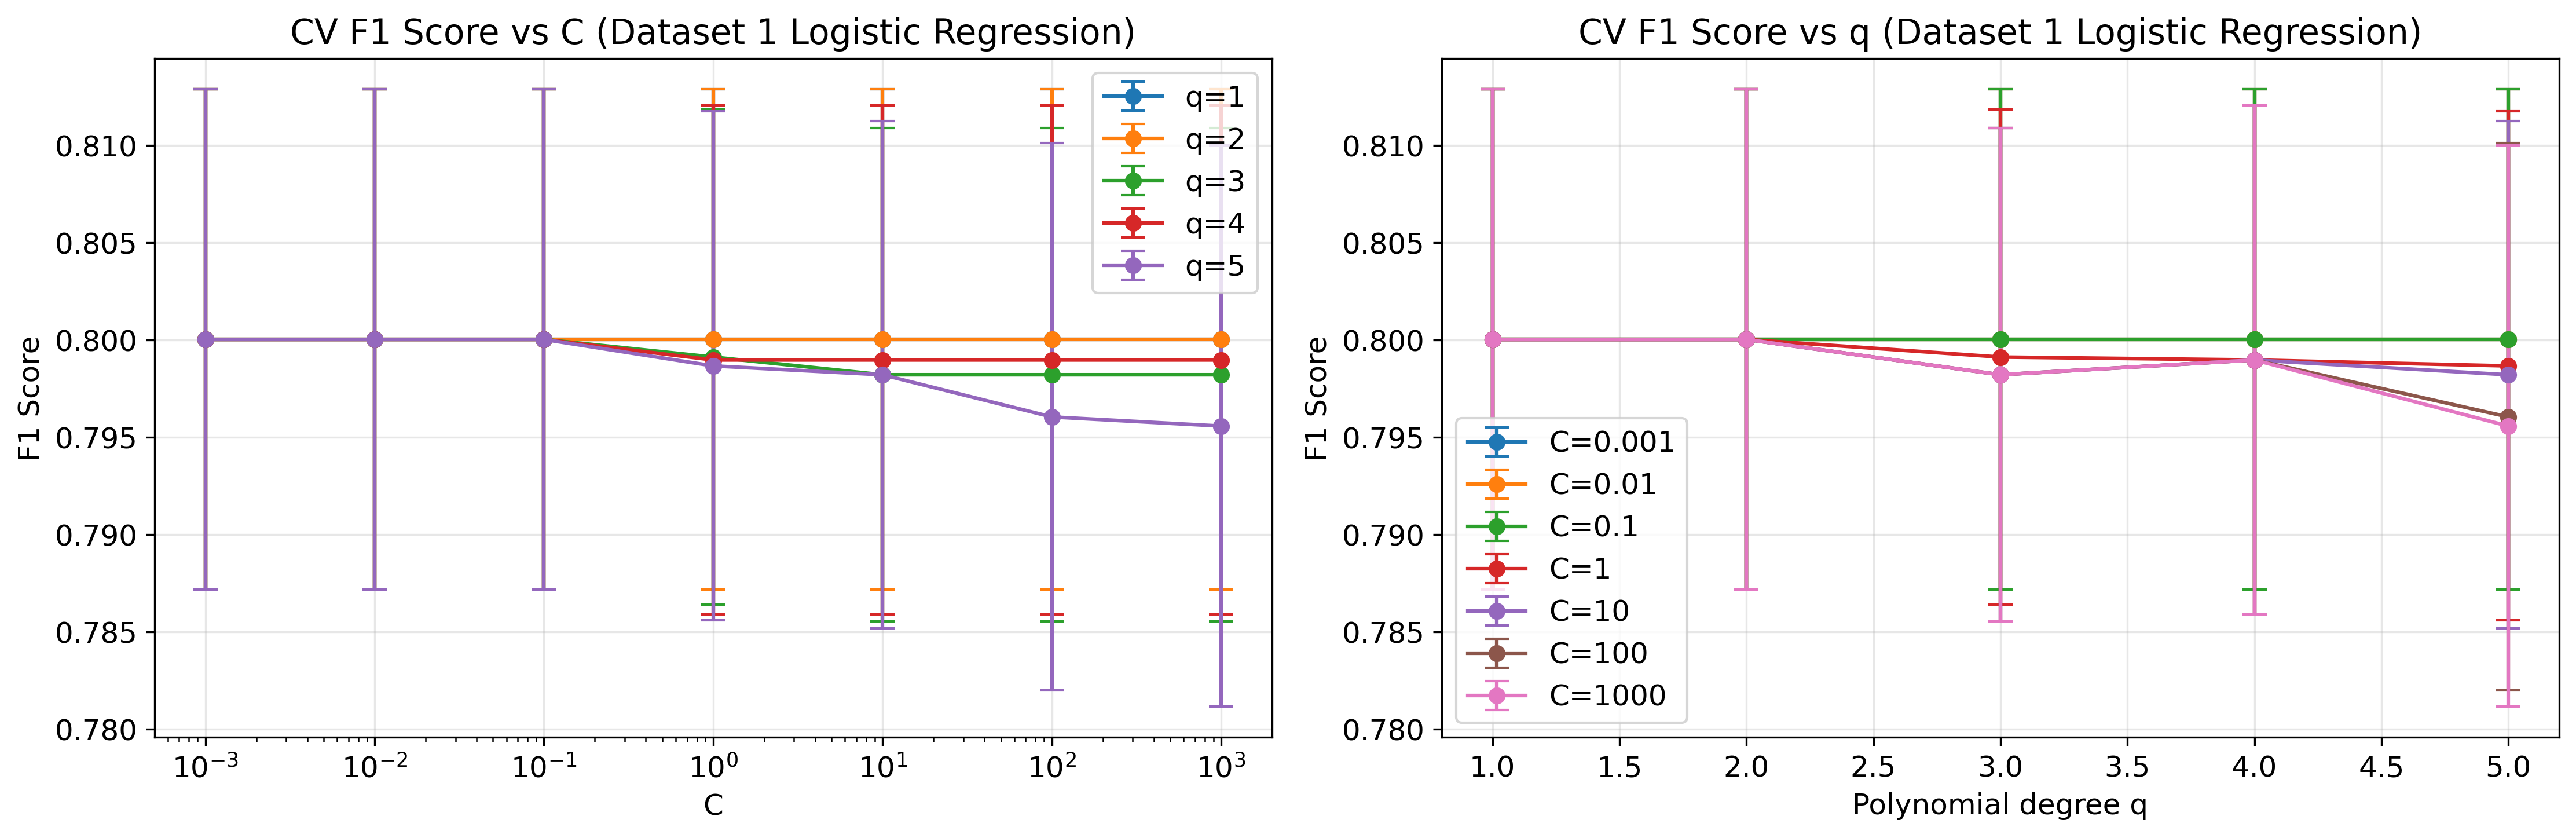
\includegraphics[width=0.7\textwidth]{figures/dataset1_logistic_cv.png}
\caption{Cross-validation results for Logistic Regression on Dataset 1. The optimal configuration is $q=1$, $C=0.001$.}
\label{fig:dataset1_logistic_cv}
\end{figure}

\subsubsection*{(ii)}

\textbf{Methodology:} Grid search over $C \in \{0.001, 0.01, 0.1, 1, 10, 100, 1000\}$ with $L_2$ penalty.

\textbf{Results:} Optimal regularization is $C=0.001$ (very strong regularization) with $q=1$, achieving CV F1=0.8000.

\textbf{Analysis:} Strong regularization (low $C$) is preferred, which typically indicates model tendency toward overfitting. But visualization of the decision boundary reveals that the model classifies class +1 for nearly all samples, and hence it is essentially replicating the most-frequent baseline classifier. This with the high regularization preference confirms that the feature space does not have discriminative capability for this classification task.

\begin{figure}[H]
\centering
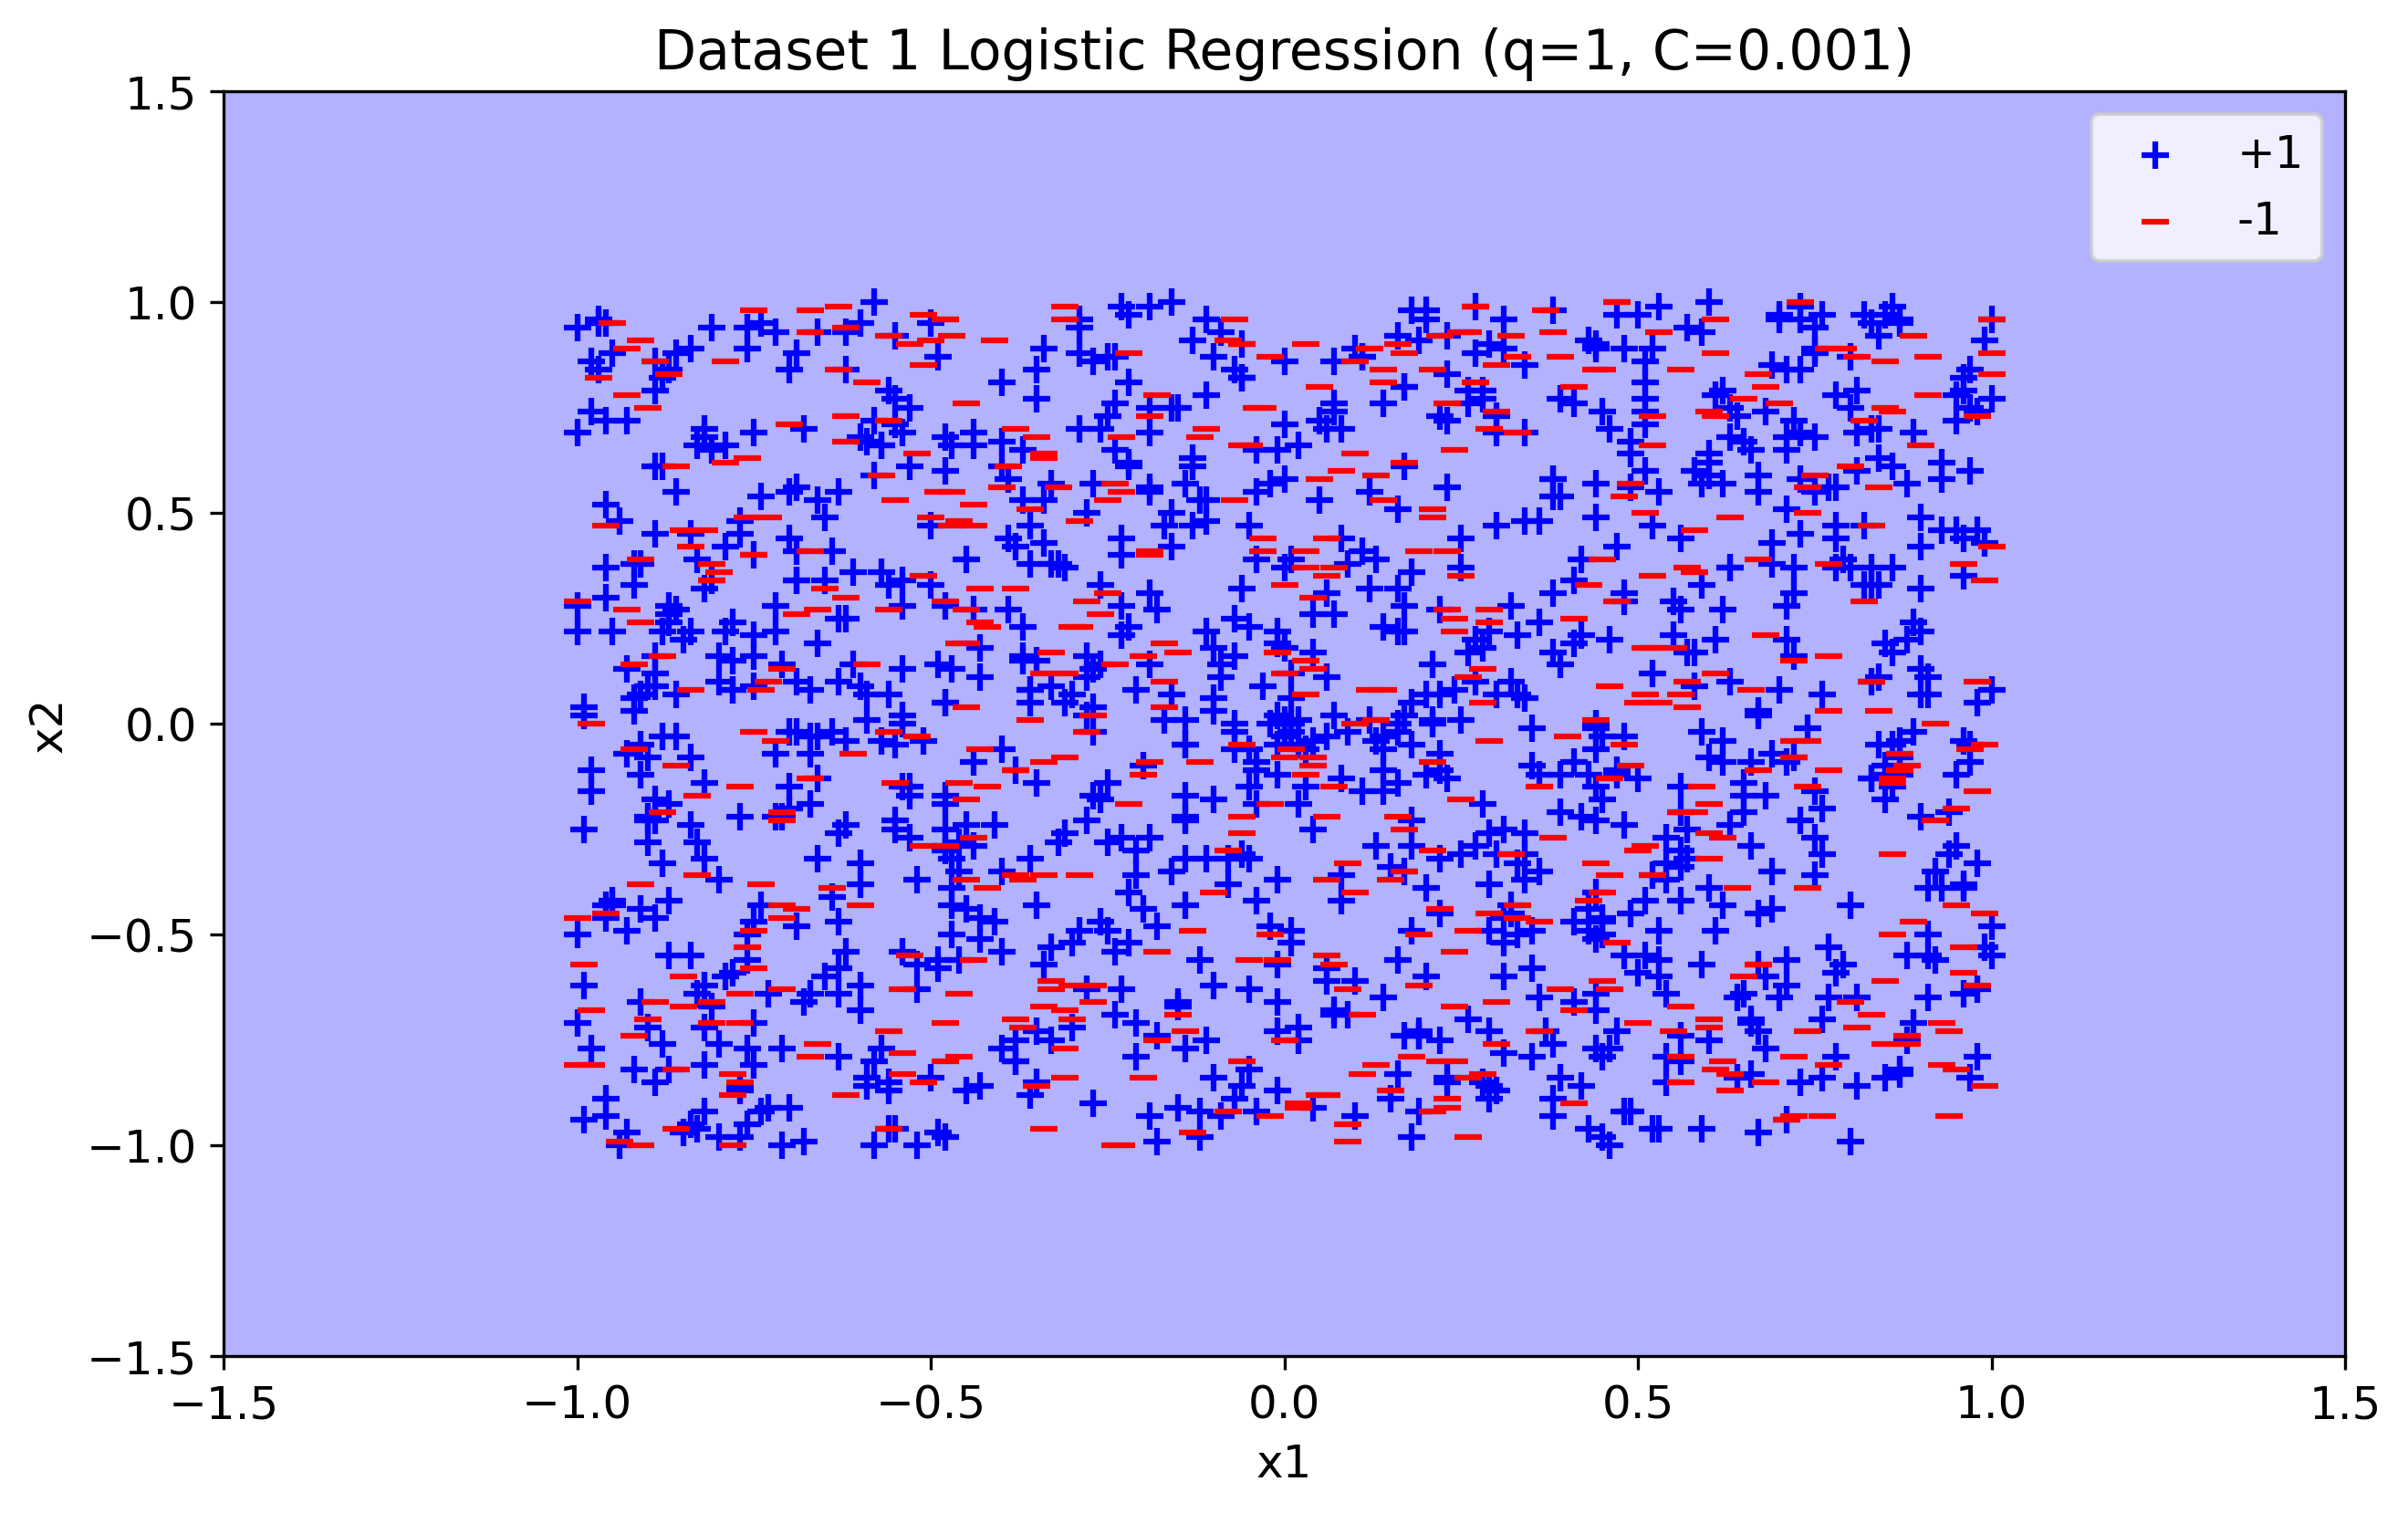
\includegraphics[width=0.55\textwidth]{figures/dataset1_logistic_boundary.png}
\caption{Dataset 1 Logistic Regression decision boundary with $q=1$, $C=0.001$.}
\label{fig:dataset1_logistic_boundary}
\end{figure}

\subsection*{(b) kNN Classifier}

\textbf{Methodology:} Used 5-fold cross-validation to select $k$ from $\{1, 3, 5, 7, 9, 11, 15, 21, 31, 41, 51\}$ with Euclidean distance metric with uniform weights.

\textbf{Results:} Optimal $k=51$ with CV F1=0.8000. The cross-validation curve illustrates monotonic improvement with larger $k$, and the performance levels off for large $k$ values. The small $k$ values perform worse, contrary to typical overfitting patterns where small $k$ yields high training accuracy.

\textbf{Interpretation:} The large optimal $k$ indicates absence of local neighborhood structure. When $k$ approaches the dataset size, kNN approximates a majority vote across the entire dataset, which explains performance equivalence with the baseline most-frequent classifier. The decision boundary with $k=51$ is highly smoothed, reflecting this global averaging behavior.

\begin{figure}[H]
\centering
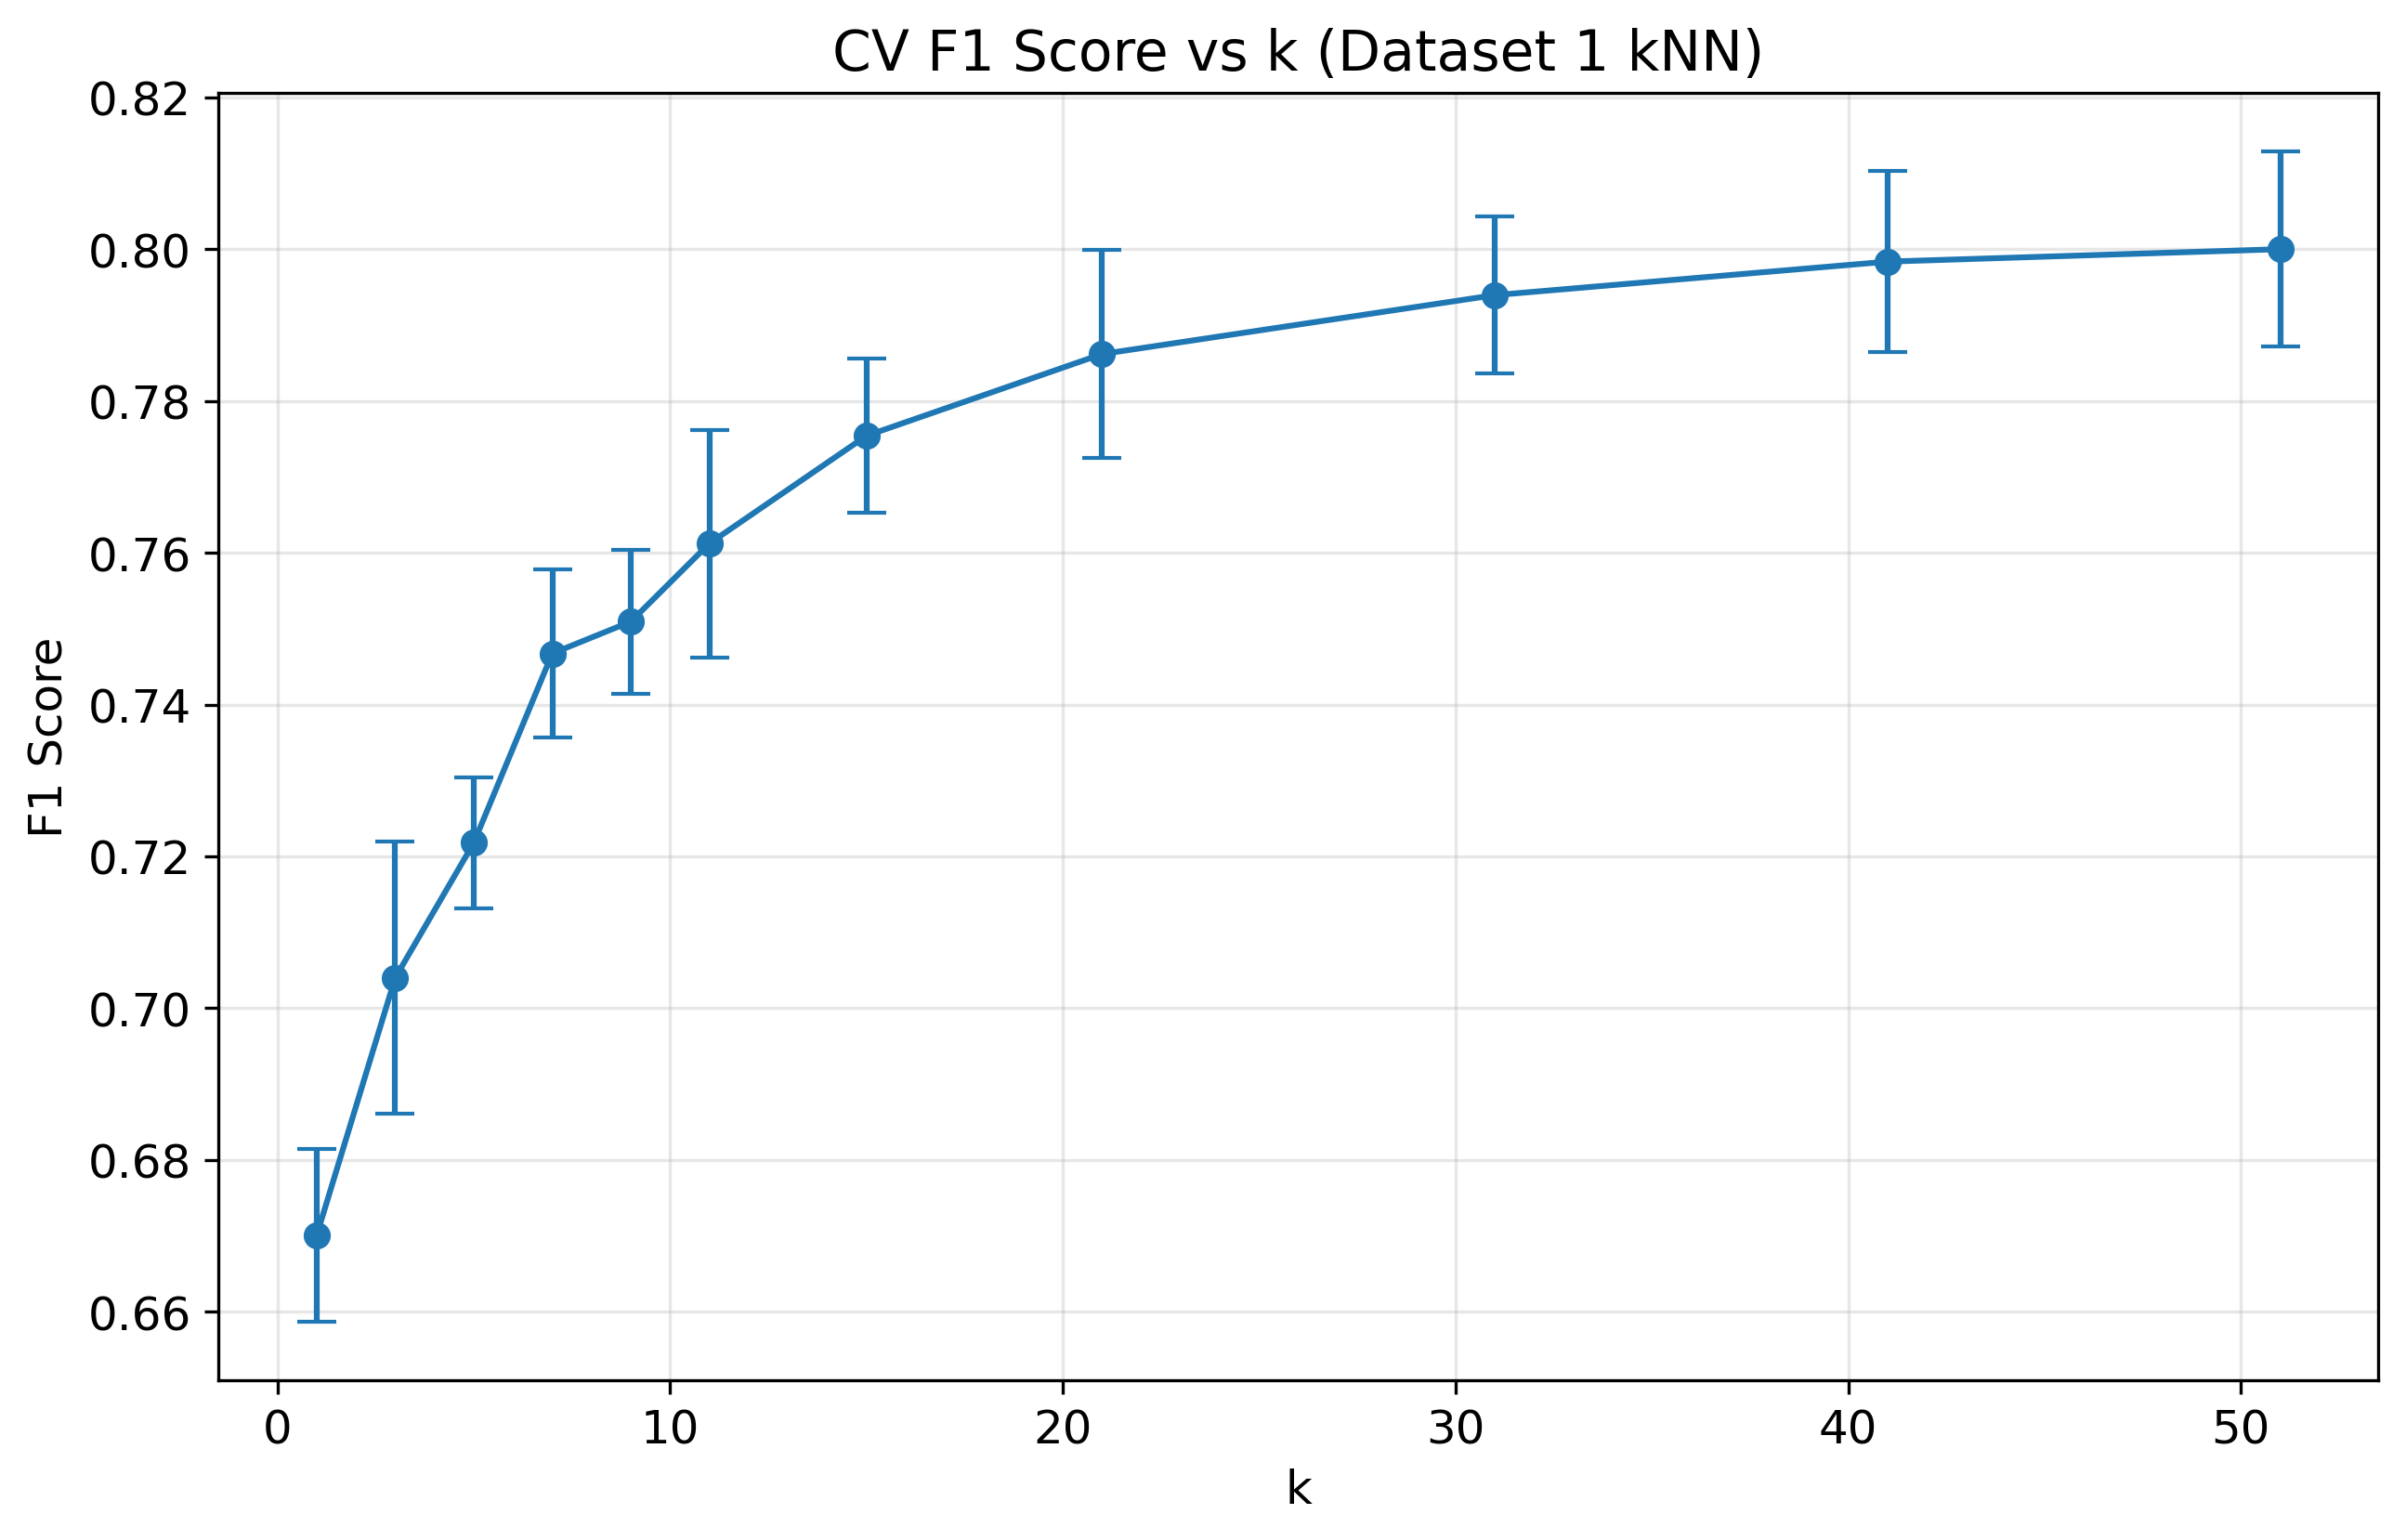
\includegraphics[width=0.5\textwidth]{figures/dataset1_knn_cv.png}
\caption{Cross validation results for kNN on Dataset 1. The optimal $k=51$.}
\label{fig:dataset1_knn_cv}
\end{figure}

\begin{figure}[H]
\centering
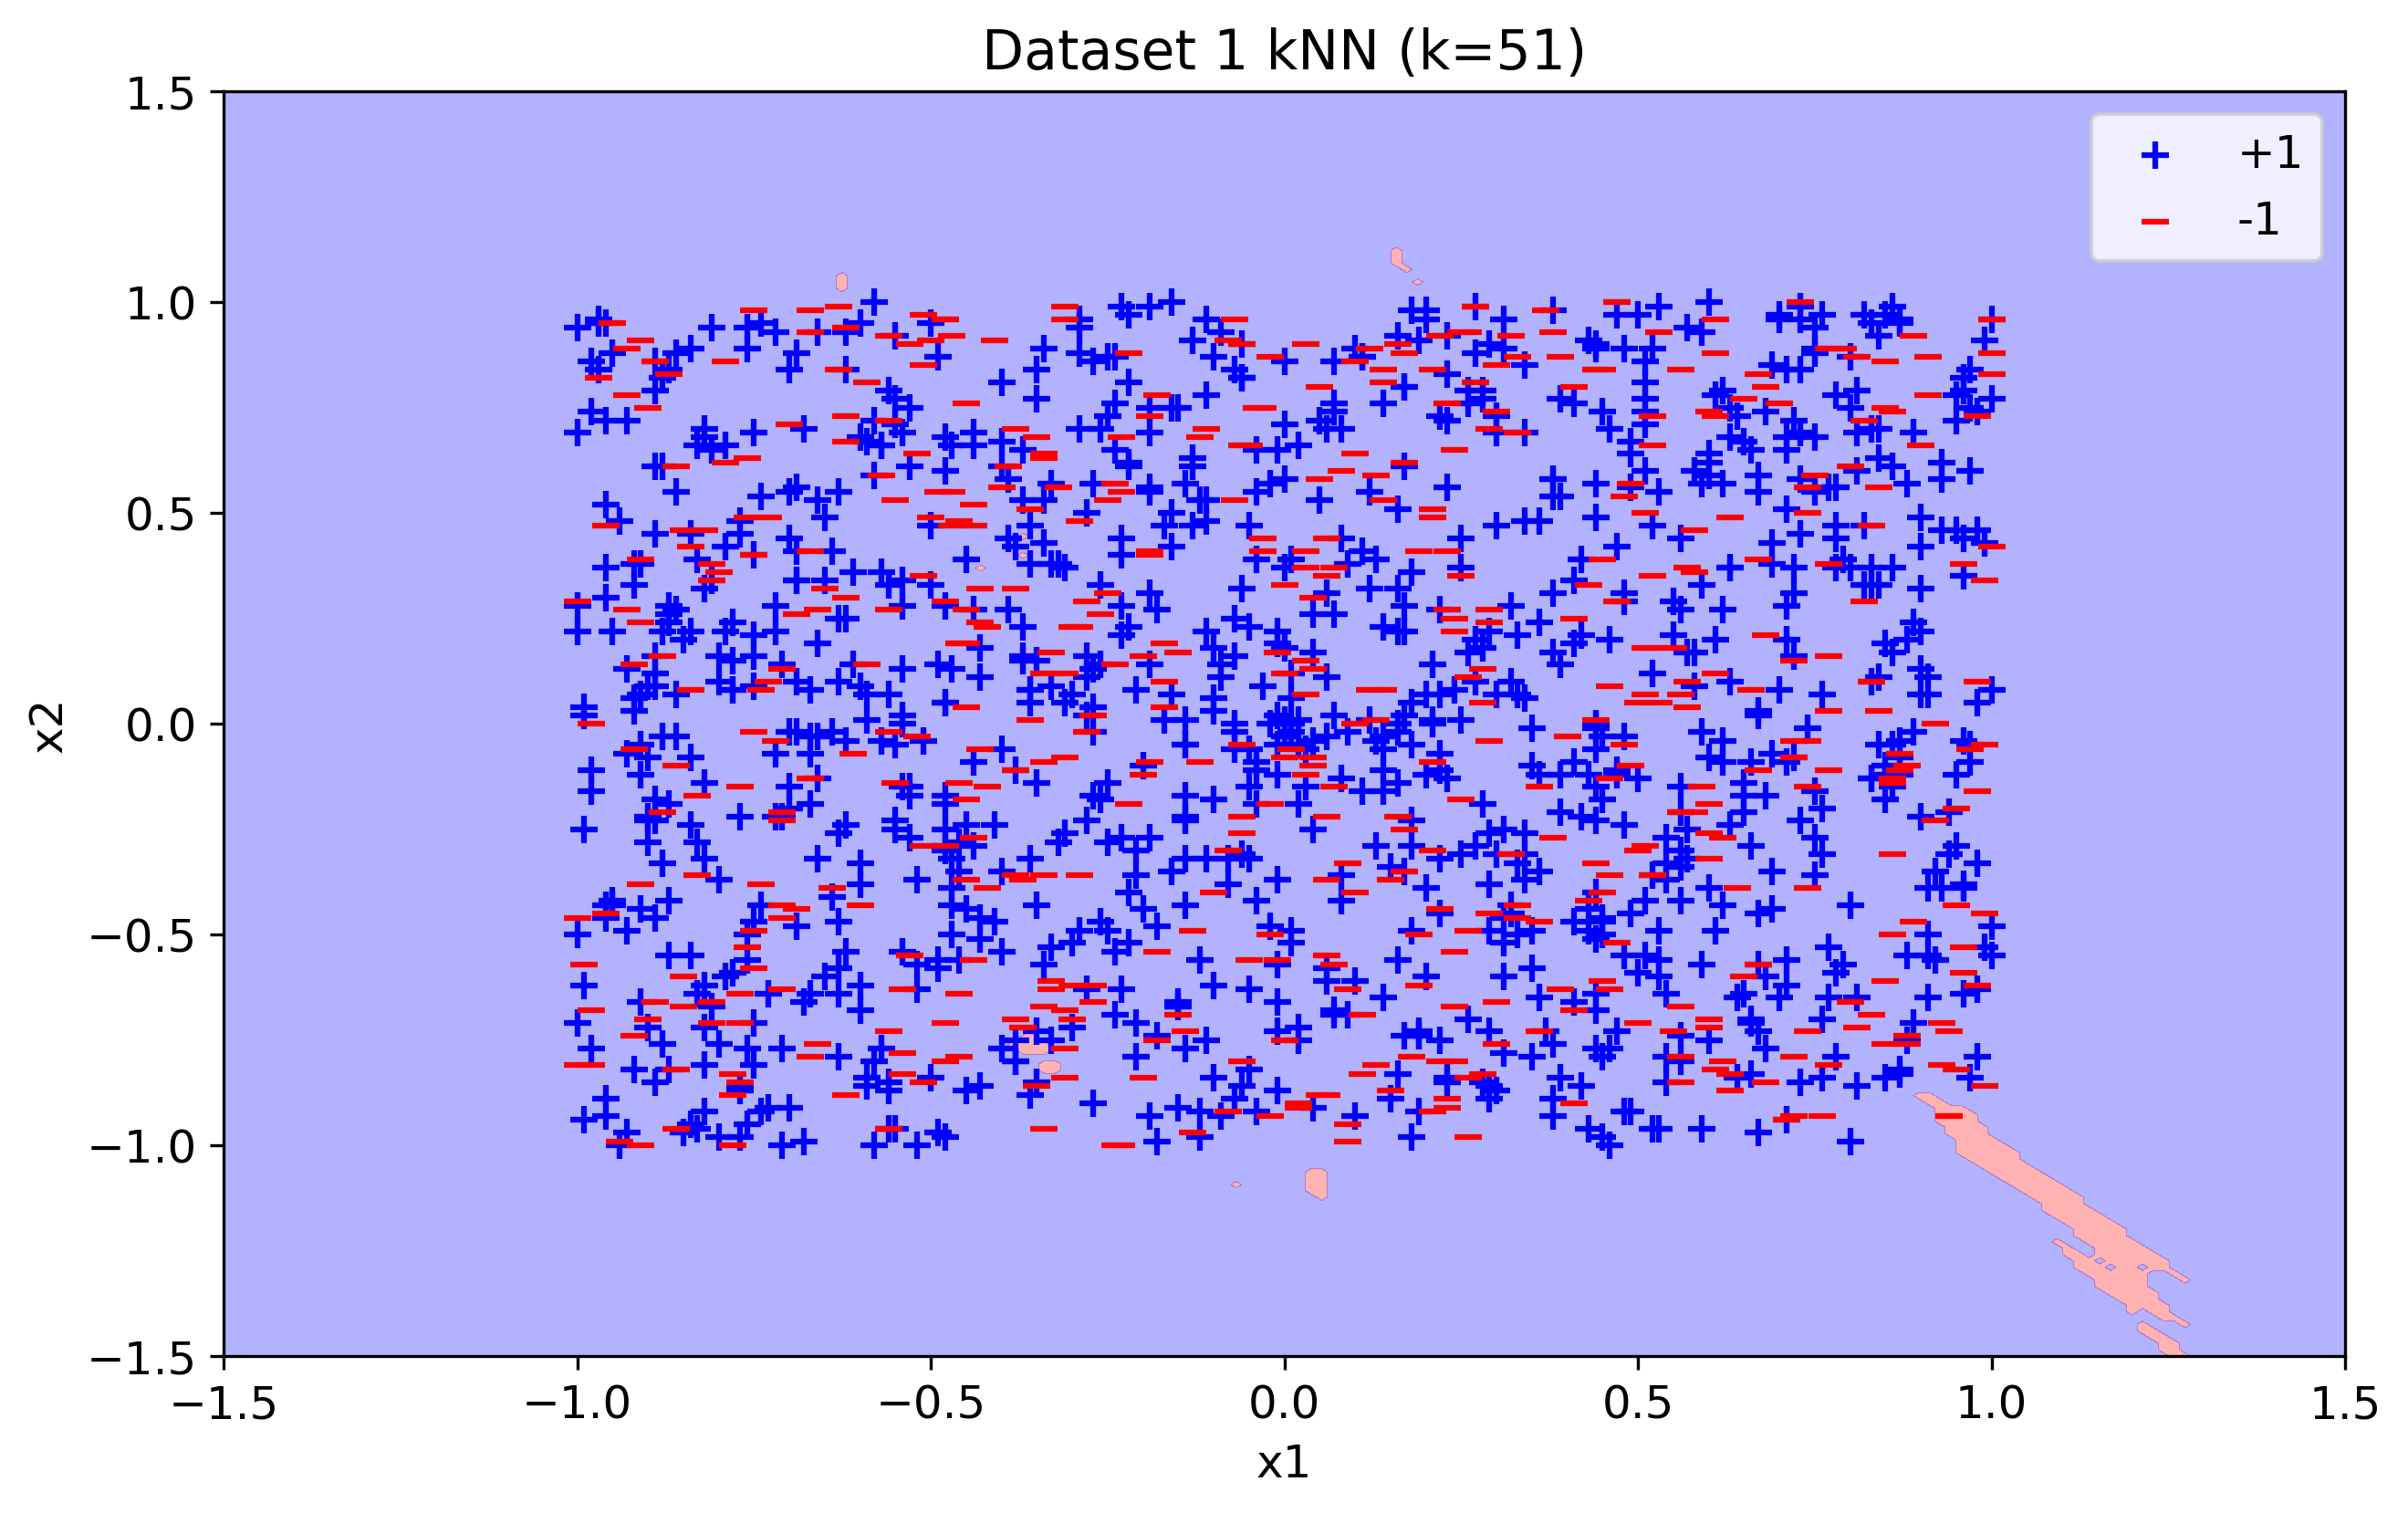
\includegraphics[width=0.5\textwidth]{figures/dataset1_knn_boundary.png}
\caption{Dataset 1 kNN decision boundary with $k=51$.}
\label{fig:dataset1_knn_boundary}
\end{figure}

\subsection*{(c) Confusion Matrices}

\textbf{Data Source:} All confusion matrices computed on full training data (not a held-out test set) by predicting labels for the same samples used during training. This approach assesses training performance and enables direct comparison with baseline classifiers.

\textbf{Logistic Regression ($q=1$, $C=0.001$):}
\begin{table}[H]
\centering
\begin{tabular}{lcc}
\toprule
 & Predicted -1 & Predicted +1 \\
\midrule
Actual -1 & 0 & 528 \\
Actual +1 & 0 & 1057 \\
\bottomrule
\end{tabular}
\end{table}
Metrics: Accuracy=0.6669, TPR=1.0, FPR=1.0, Precision=0.6669

\textbf{kNN ($k=51$):}
\begin{table}[H]
\centering
\begin{tabular}{lcc}
\toprule
 & Predicted -1 & Predicted +1 \\
\midrule
Actual -1 & 1 & 527 \\
Actual +1 & 0 & 1057 \\
\bottomrule
\end{tabular}
\end{table}
Metrics: Accuracy=0.6675, TPR=1.0, FPR=0.9981, Precision=0.6673

\textbf{Baseline Most Frequent:}
\begin{table}[H]
\centering
\begin{tabular}{lcc}
\toprule
 & Predicted -1 & Predicted +1 \\
\midrule
Actual -1 & 0 & 528 \\
Actual +1 & 0 & 1057 \\
\bottomrule
\end{tabular}
\end{table}
Metrics: Accuracy=0.6669

\textbf{Baseline Random (uniform):}
\begin{table}[H]
\centering
\begin{tabular}{lcc}
\toprule
 & Predicted -1 & Predicted +1 \\
\midrule
Actual -1 & 253 & 275 \\
Actual +1 & 543 & 514 \\
\bottomrule
\end{tabular}
\end{table}
Metrics: Accuracy=0.4839

\textbf{Confusion Matrix Calculation:} Each matrix element represents: TN (True Negatives) = correct -1 predictions; FP (False Positives) = incorrect +1 predictions; FN (False Negatives) = incorrect -1 predictions; TP (True Positives) = correct +1 predictions. Computed using \texttt{sklearn.metrics.confusion\_matrix} with labels=[-1, 1].

\subsection*{(d) ROC Curves}

\textbf{Methodology:} ROC curves generated by varying classification threshold over model confidence scores. For Logistic Regression, used \texttt{decision\_function()} output; for kNN, used \texttt{predict\_proba()}. Computed using \texttt{sklearn.metrics.roc\_curve} which automatically generates threshold sweep. Baseline classifiers plotted as single points at their fixed (FPR, TPR) coordinates.

\textbf{Results:}
\begin{itemize}
    \item Logistic Regression: AUC=0.5045
    \item kNN: AUC=0.5686
    \item Most Frequent Baseline: point at (1.0, 1.0)
    \item Random Baseline: point near (0.5, 0.5)
\end{itemize}

\textbf{Observations:} Both ROC curves closely follow the 45° diagonal representing random classification. The trained classifiers show minimal improvement over random chance (AUC $\approx$ 0.5), with sufficient detail points to reveal curve shape. The most-frequent baseline appears at (1,1) because it predicts all positive, yielding TPR=1 and FPR=1.

\begin{figure}[H]
\centering
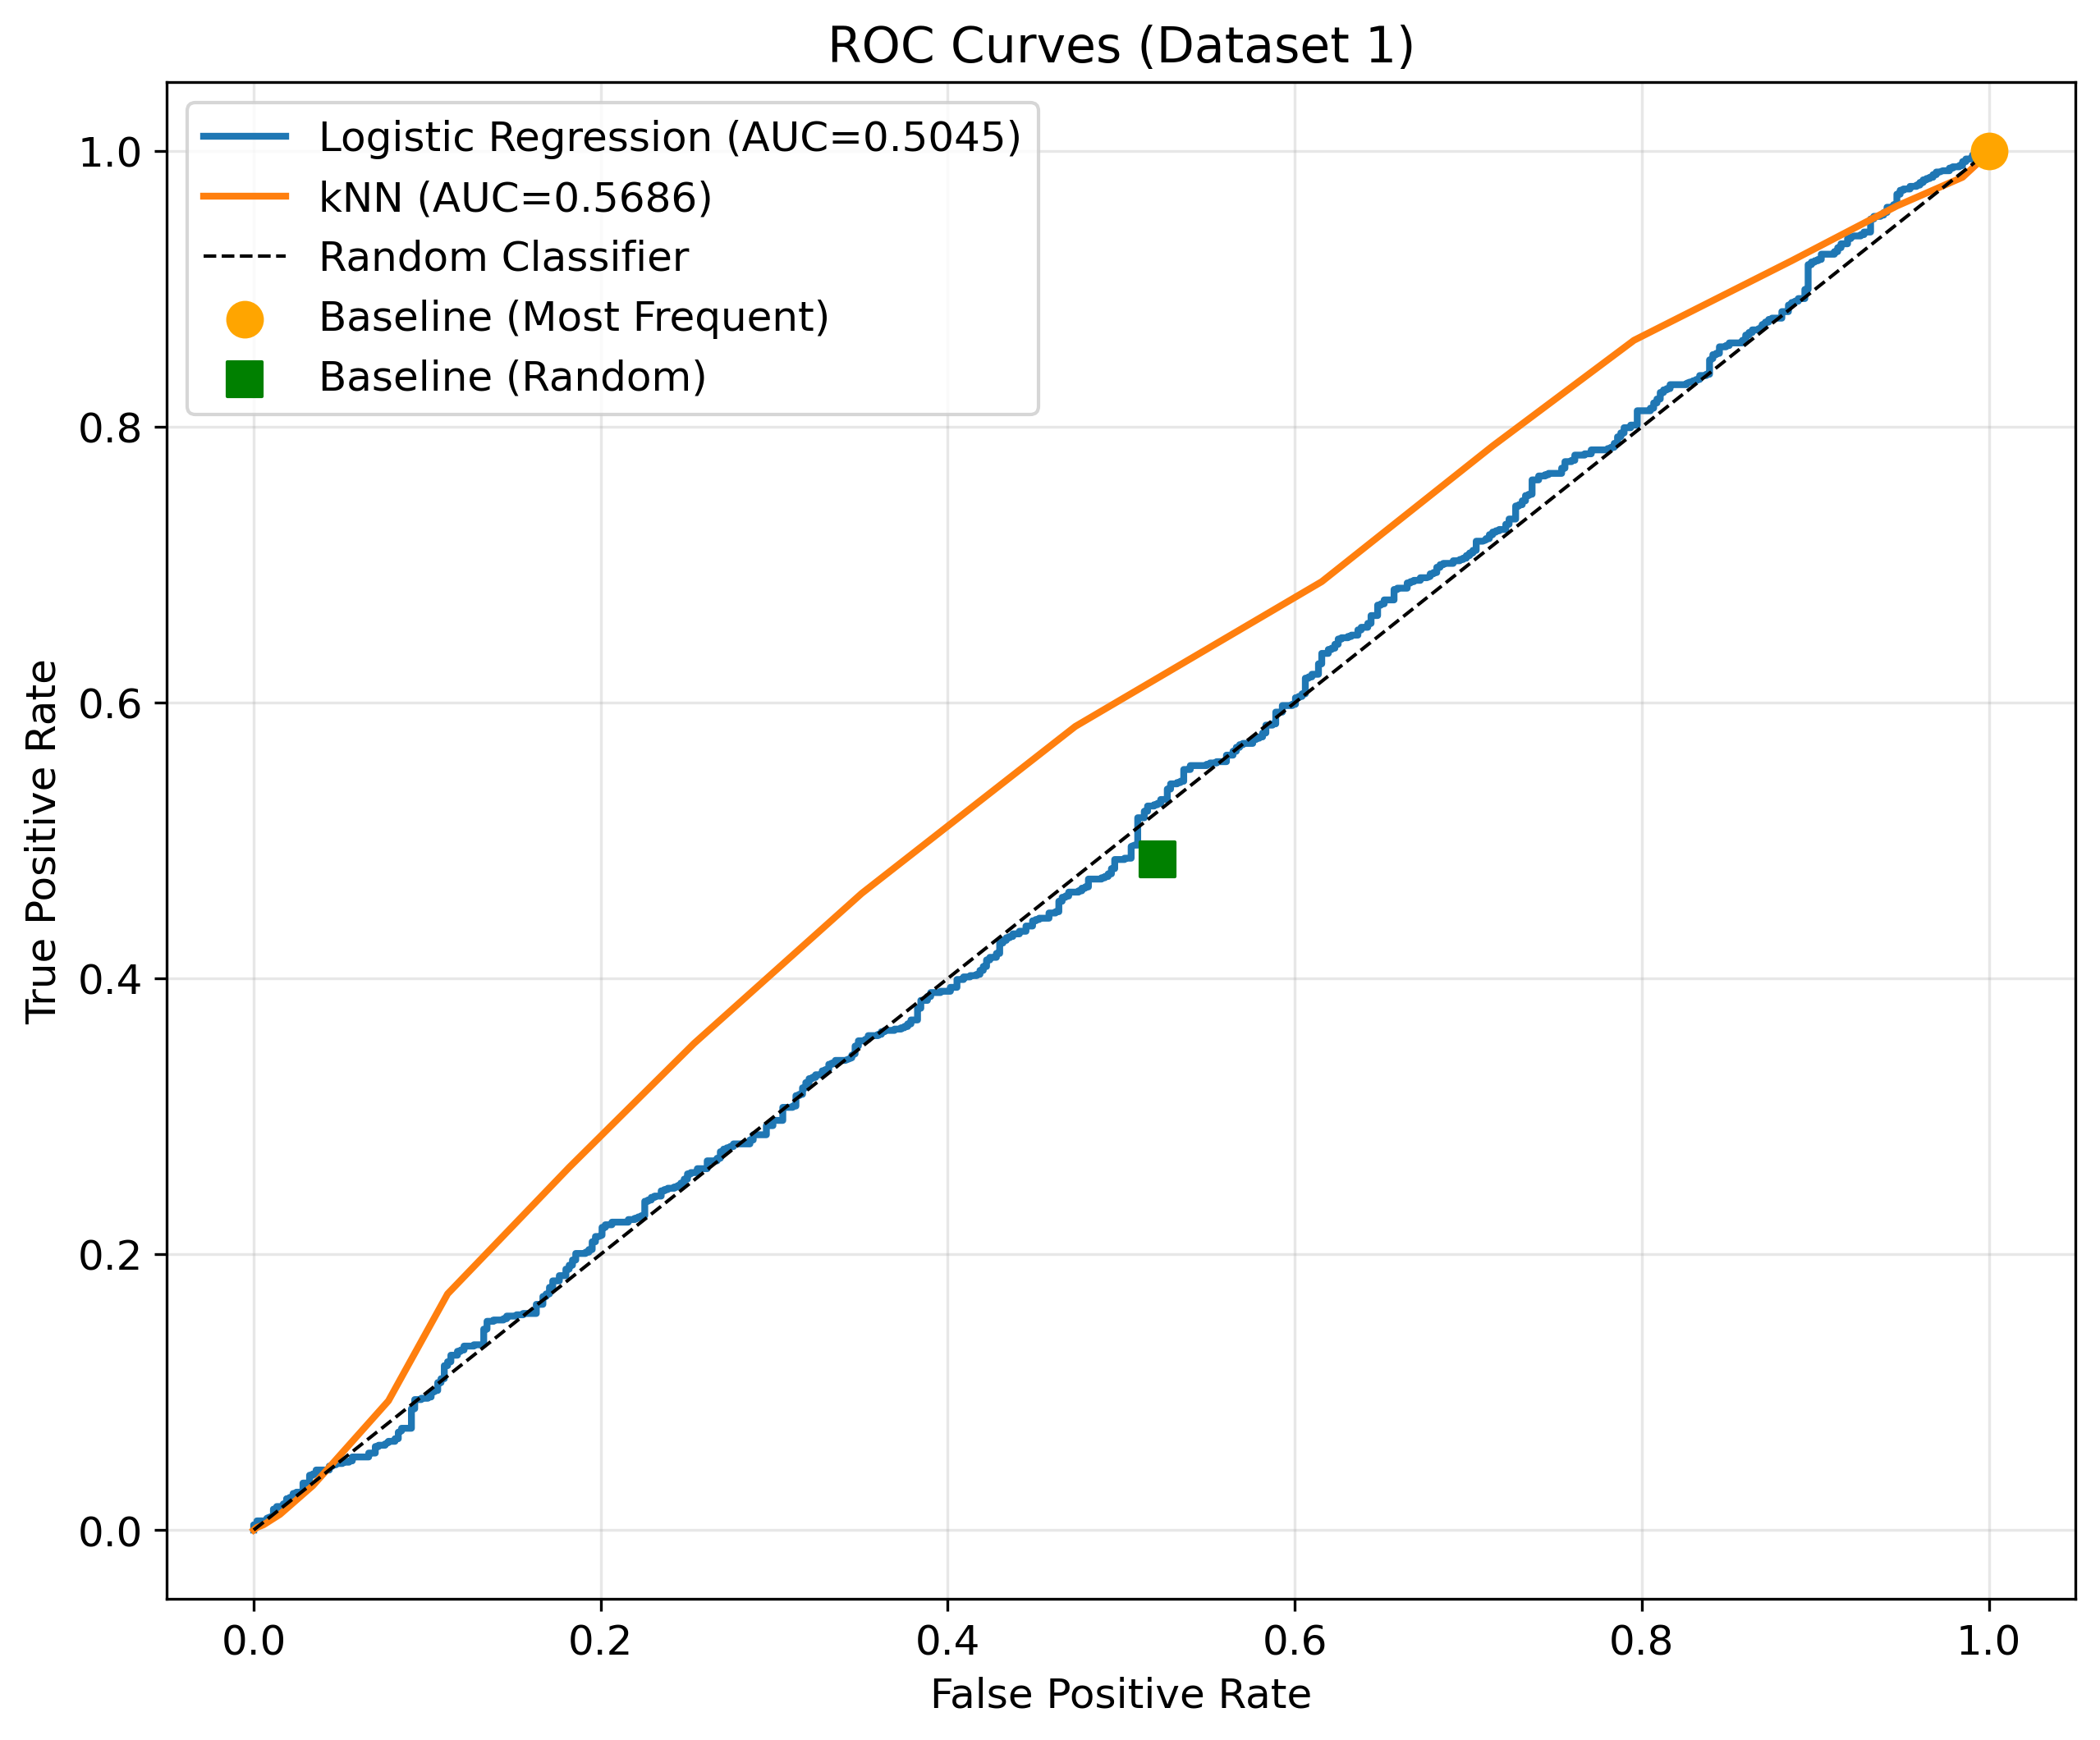
\includegraphics[width=0.5\textwidth]{figures/dataset1_roc.png}
\caption{ROC curves for Dataset 1.}
\label{fig:dataset1_roc}
\end{figure}

\subsection*{(e) Performance Evaluation and Comparison}

\textbf{Statistical Performance:} Both trained classifiers achieve AUC marginally above 0.5 (random classifier), with kNN showing slight advantage (AUC=0.5686 vs 0.5045). But this difference is not practically significant given both values' proximity to random performance.

\textbf{Comparison with Baselines:} Logistic Regression exactly replicates most-frequent baseline behavior (Accuracy=0.6669 for both). kNN shows negligible improvement (Accuracy=0.6675), making only one negative prediction across 1585 samples. Both outperform random baseline by $\sim$18 percentage points, but this improvement stems entirely from exploiting class imbalance rather than learning decision boundaries.

\textbf{ROC Analysis:} The ROC curves' position along the diagonal demonstrates that varying classification thresholds does not improve the true positive rate without proportionally increasing false positives. An effective classifier would show curves bowing toward the upper-left corner (0,1). The result suggests that both models lack discrimination capacity for distinguishing between classes at any operating point.

\textbf{Recommendation:} Neither of the classifiers is deployment-ready. The data feature space lacks sufficient data to discriminate between the classes. The measured features are either uninformative or the classes overlap entirely in this representation. Collection of additional features or alternative data sources would be necessary before meaningful classification becomes possible.

\textbf{Root Cause:} The scatter plot analysis shows large class overlap in the 2D feature space, which describes the bad separability. The consistent prediction of the majority class by regularized models suggests no learnable patterns exist in the current feature representation.

\section*{(ii) Dataset 2}

\subsection*{(a)}

\subsubsection*{(i)}

\textbf{Methodology:} Same cross validation framework as Dataset 1: 5-fold CV, F1 score metric, $q \in \{1, 2, 3, 4, 5\}$.

\textbf{Results:} Optimal polynomial degree $q=2$ (quadratic features) with CV F1=0.9508. Cross-validation plots show that $q=2$ dominates across most $C$ values, with $q=3,4,5$ showing no additional benefit and $q=1$ underperforming significantly.

\textbf{Interpretation:} The quadratic optimum indicates genuine nonlinear class separation. The clear performance improvement over linear ($q=1$) followed by plateau at higher orders suggests the true decision boundary is approximately quadratic. This dataset's structure is well behaved since the higher polynomials don't overfit.

\begin{figure}[H]
\centering
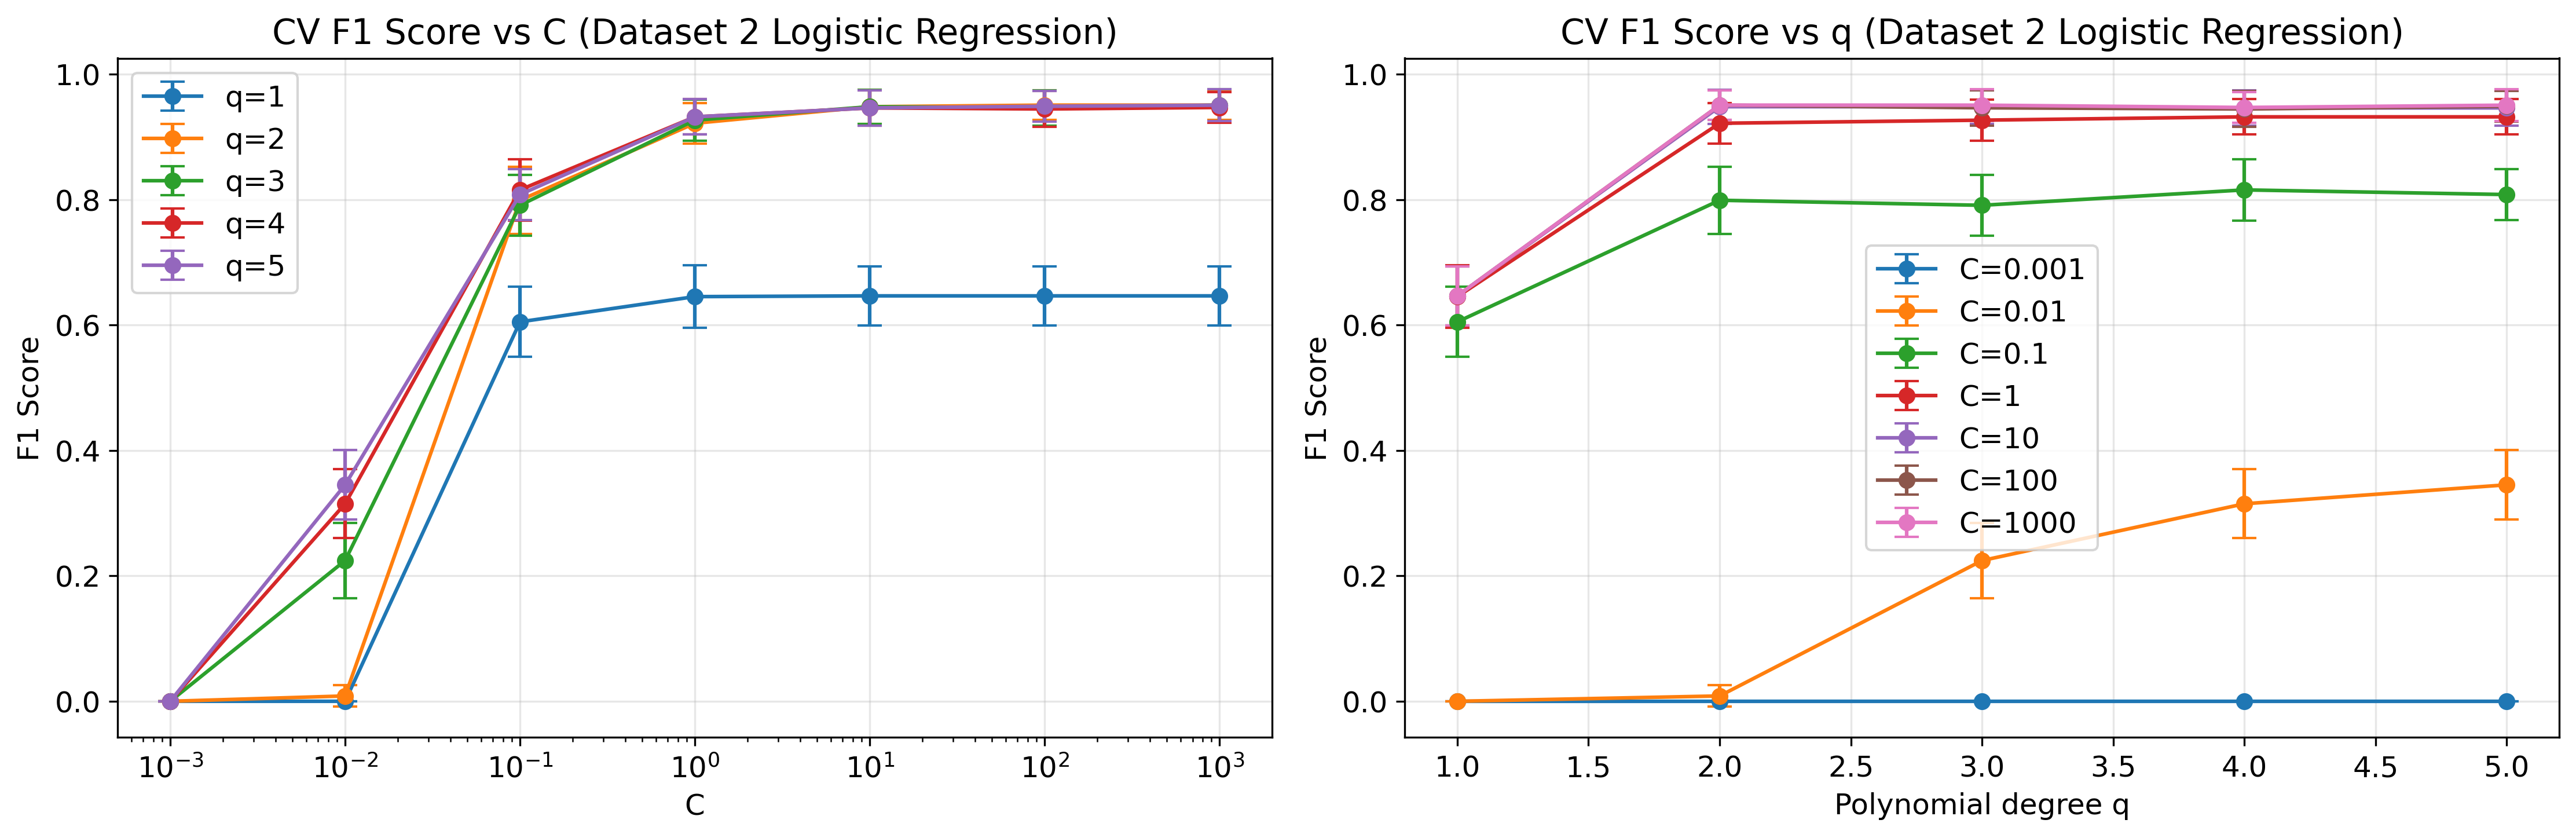
\includegraphics[width=0.7\textwidth]{figures/dataset2_logistic_cv.png}
\caption{Cross-validation results for Logistic Regression on Dataset 2. The optimal configuration is $q=2$, $C=100$.}
\label{fig:dataset2_logistic_cv}
\end{figure}

\subsubsection*{(ii)}

\textbf{Results:} Optimal $C=100$ (weak regularization) with $q=2$, achieving CV F1=0.9508.

\textbf{Analysis:} Weak regularization preference indicates the model does not tend to overfit despite using quadratic features. This behavior arises when the true underlying relationship matches the model capacity (quadratic). The decision boundary visualization confirms a smooth curved boundary that cleanly separates classes without excessive complexity.

\begin{figure}[H]
\centering
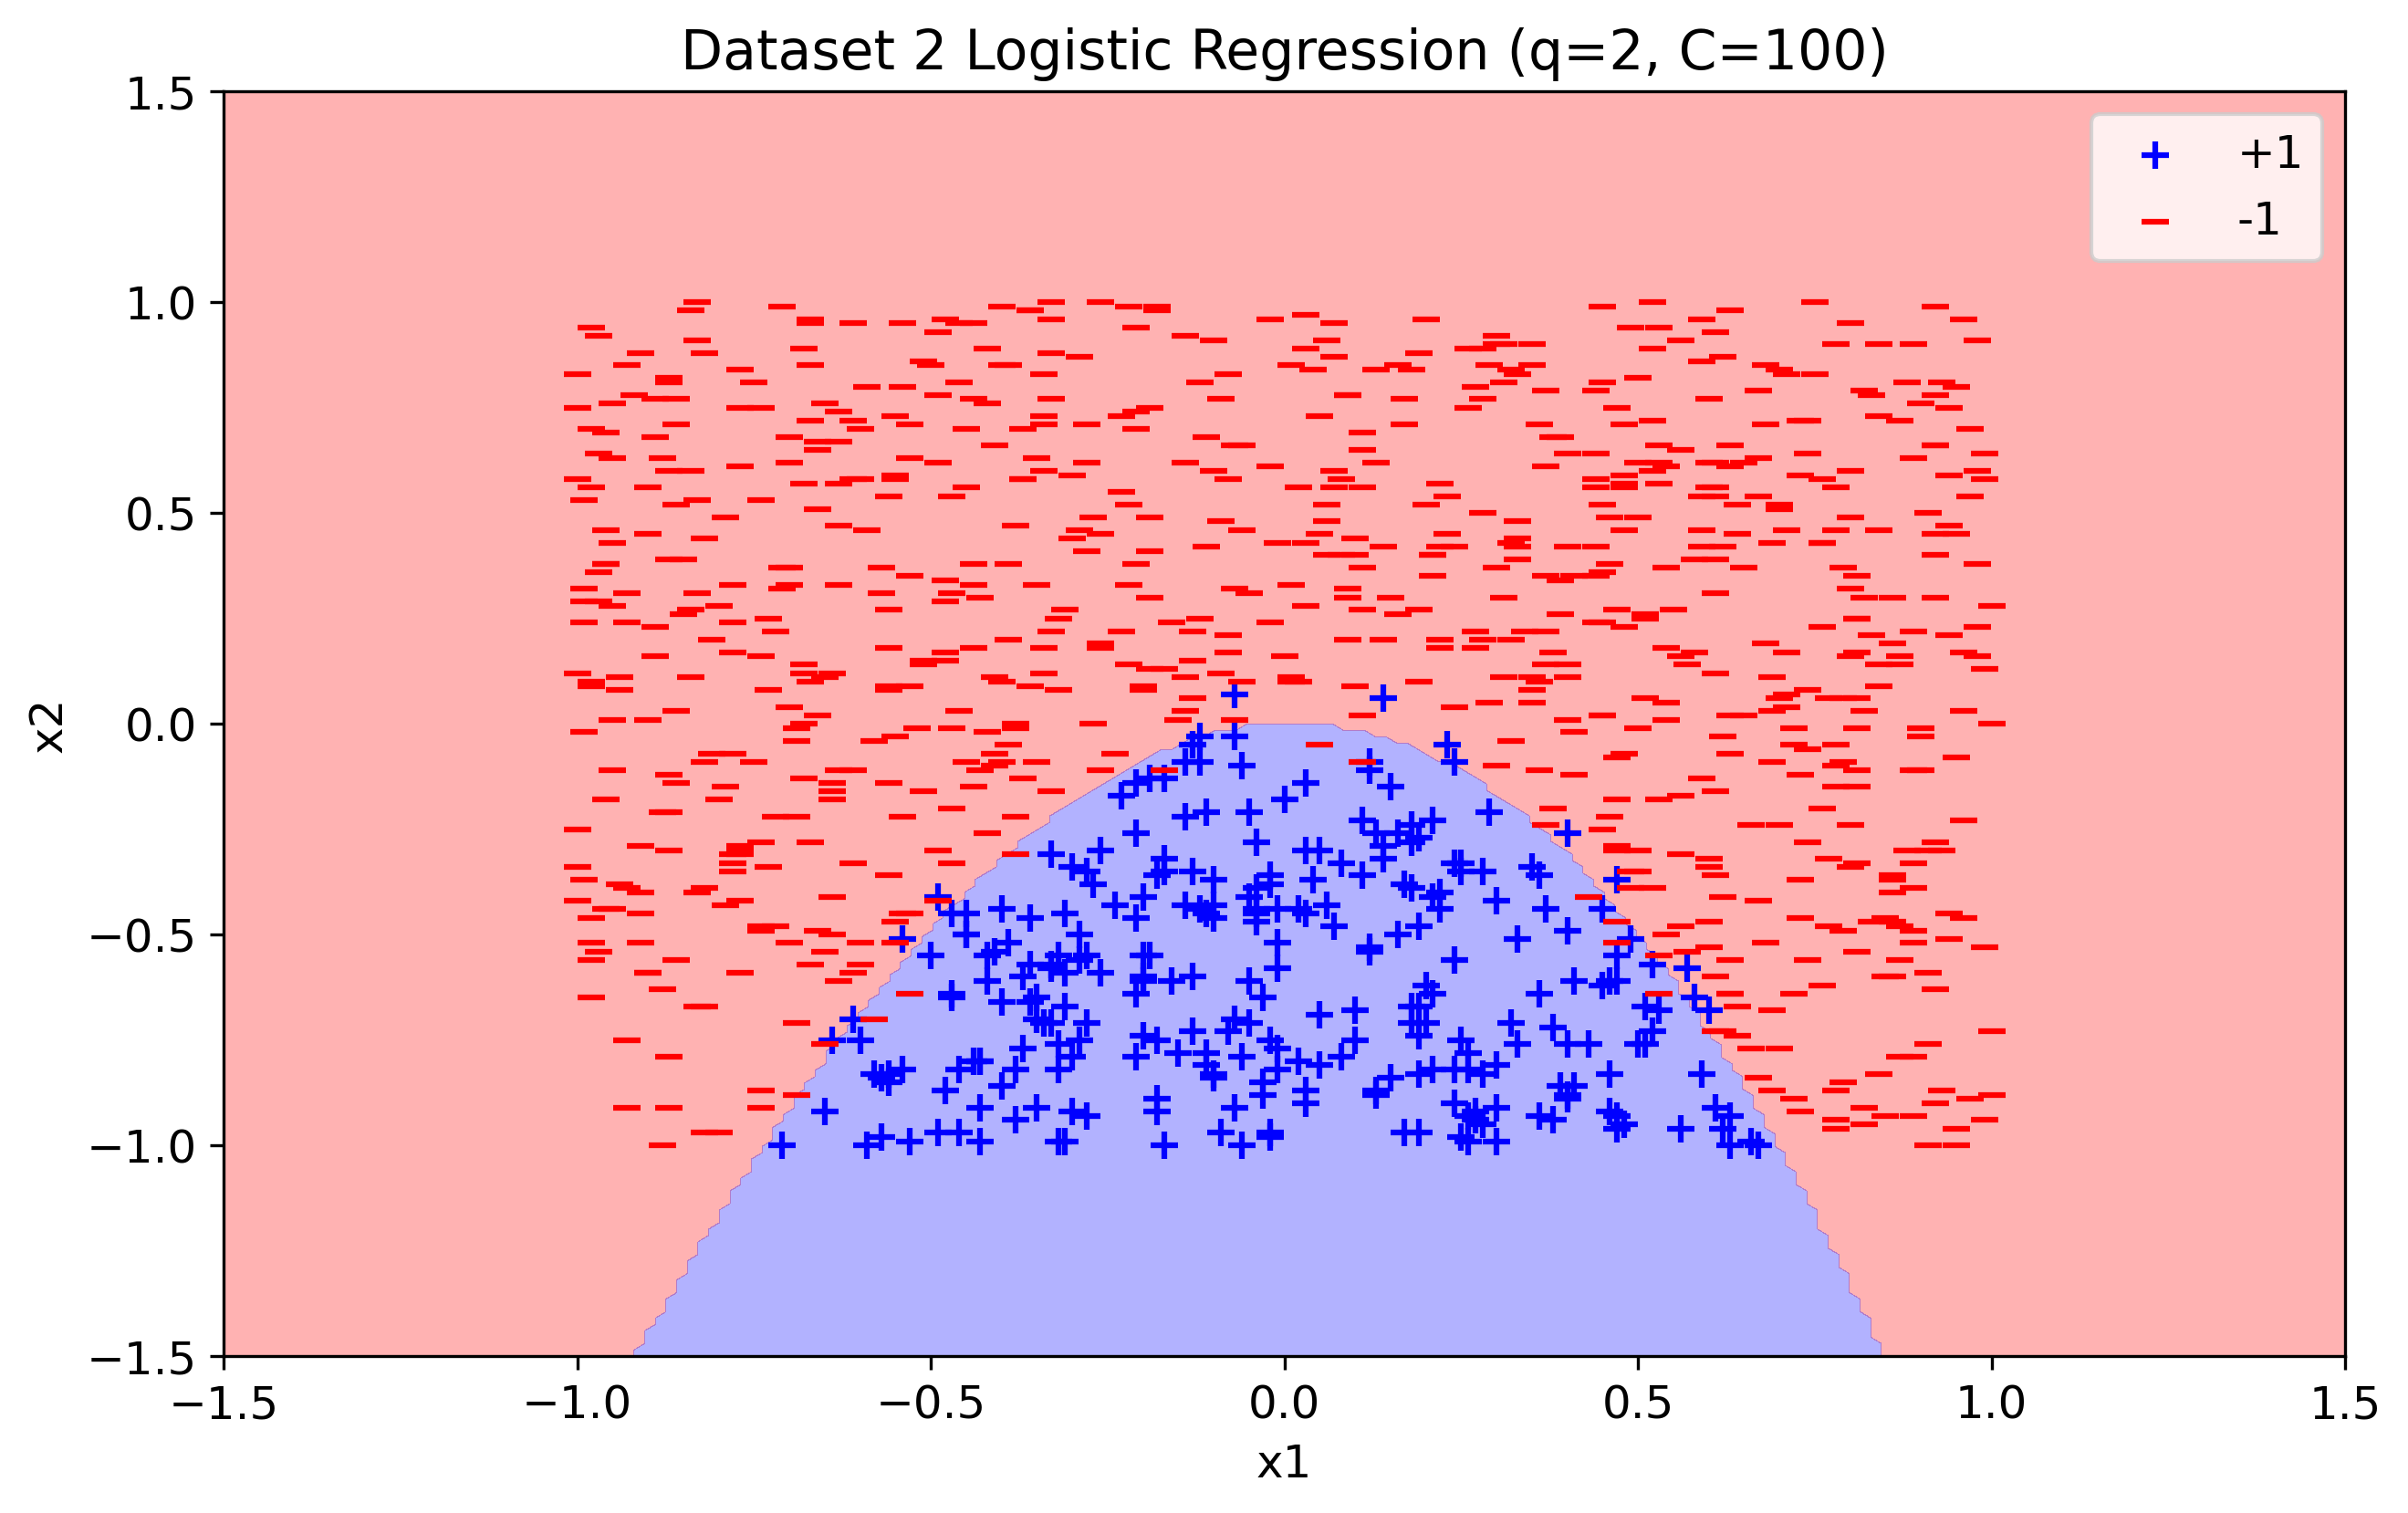
\includegraphics[width=0.55\textwidth]{figures/dataset2_logistic_boundary.png}
\caption{Dataset 2 Logistic Regression decision boundary with $q=2$, $C=100$.}
\label{fig:dataset2_logistic_boundary}
\end{figure}

\subsection*{(b)}

\textbf{Methodology:} Same k-fold CV framework as Dataset 1, testing $k \in \{1, 3, 5, 7, 9, 11, 15, 21, 31, 41, 51\}$.

\textbf{Results:} Optimal $k=7$ with CV F1=0.9498. Cross-validation curve shows peak performance at $k=7$ with smooth decline for lower $k$ (overfitting) and higher $k$ (over-smoothing)

\textbf{Interpretation:} The small optimal $k$ confirms strong local structure—nearby points share class labels. The well-defined optimum and symmetric performance degradation indicate the dataset exhibits clear neighborhood-based patterns suitable for kNN classification. The decision boundary captures complex nonlinear structure while maintaining generalization.

\begin{figure}[H]
\centering
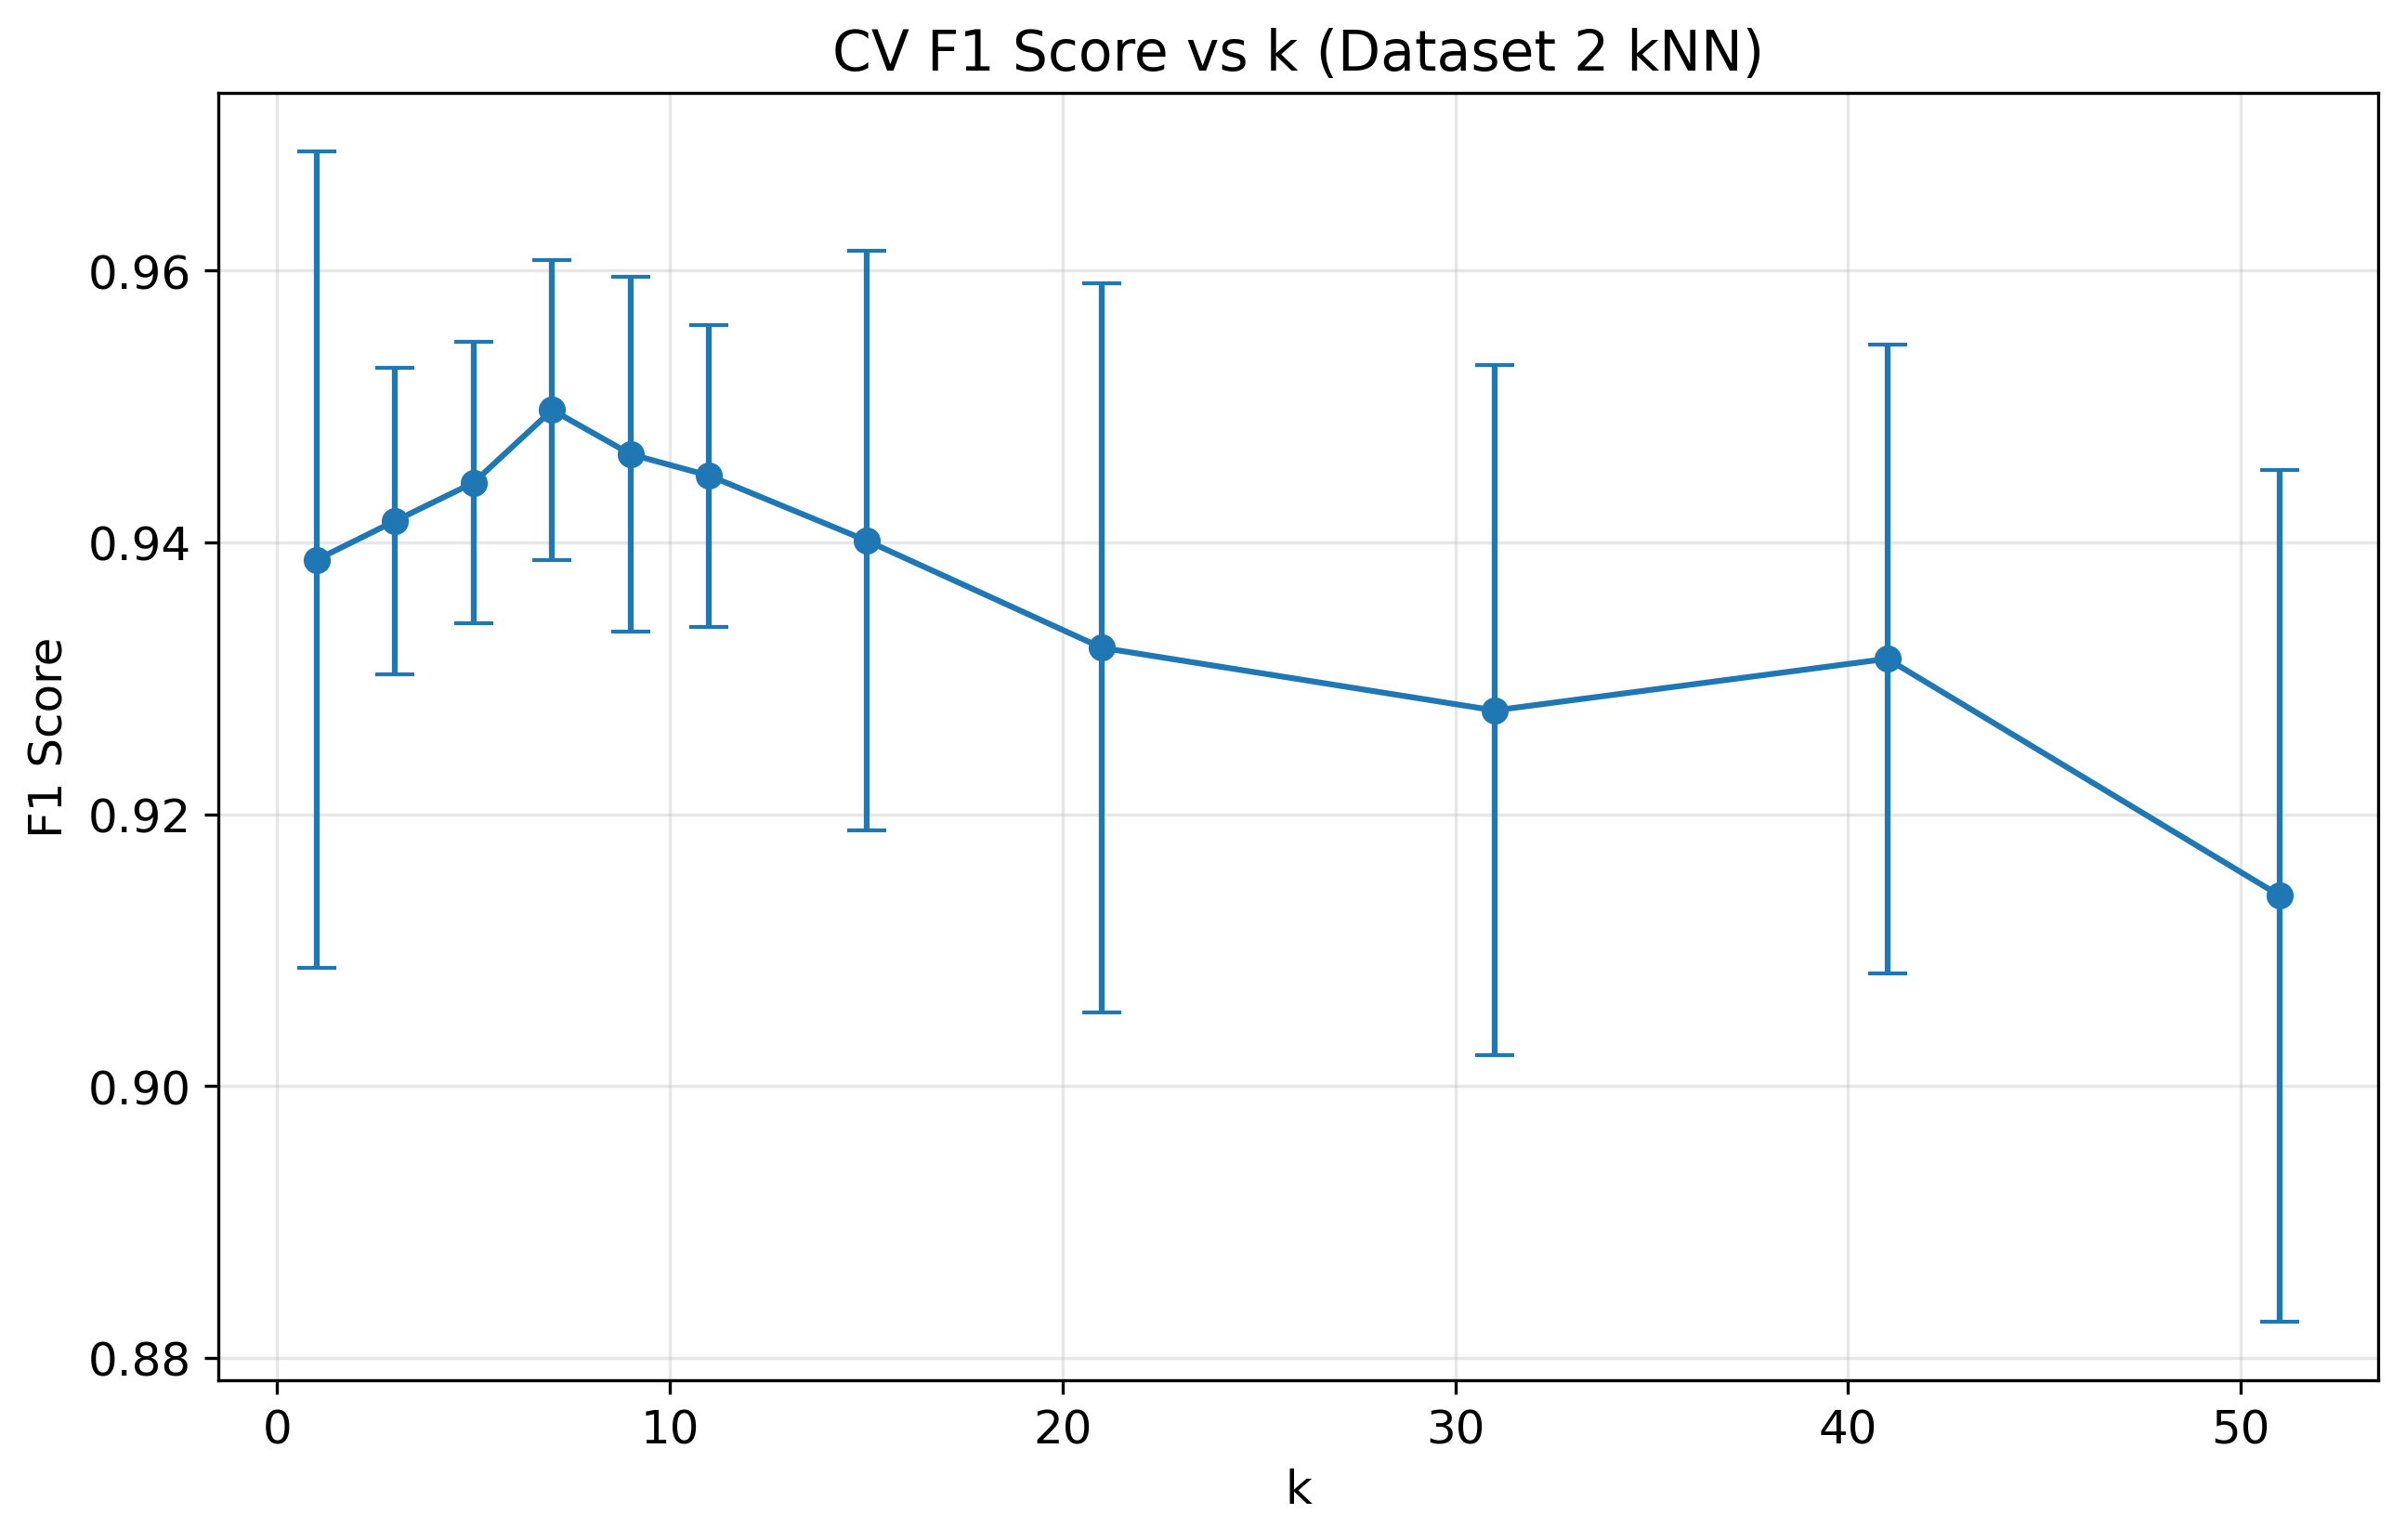
\includegraphics[width=0.5\textwidth]{figures/dataset2_knn_cv.png}
\caption{Cross-validation results for kNN on Dataset 2. The optimal $k=7$.}
\label{fig:dataset2_knn_cv}
\end{figure}

\begin{figure}[H]
\centering
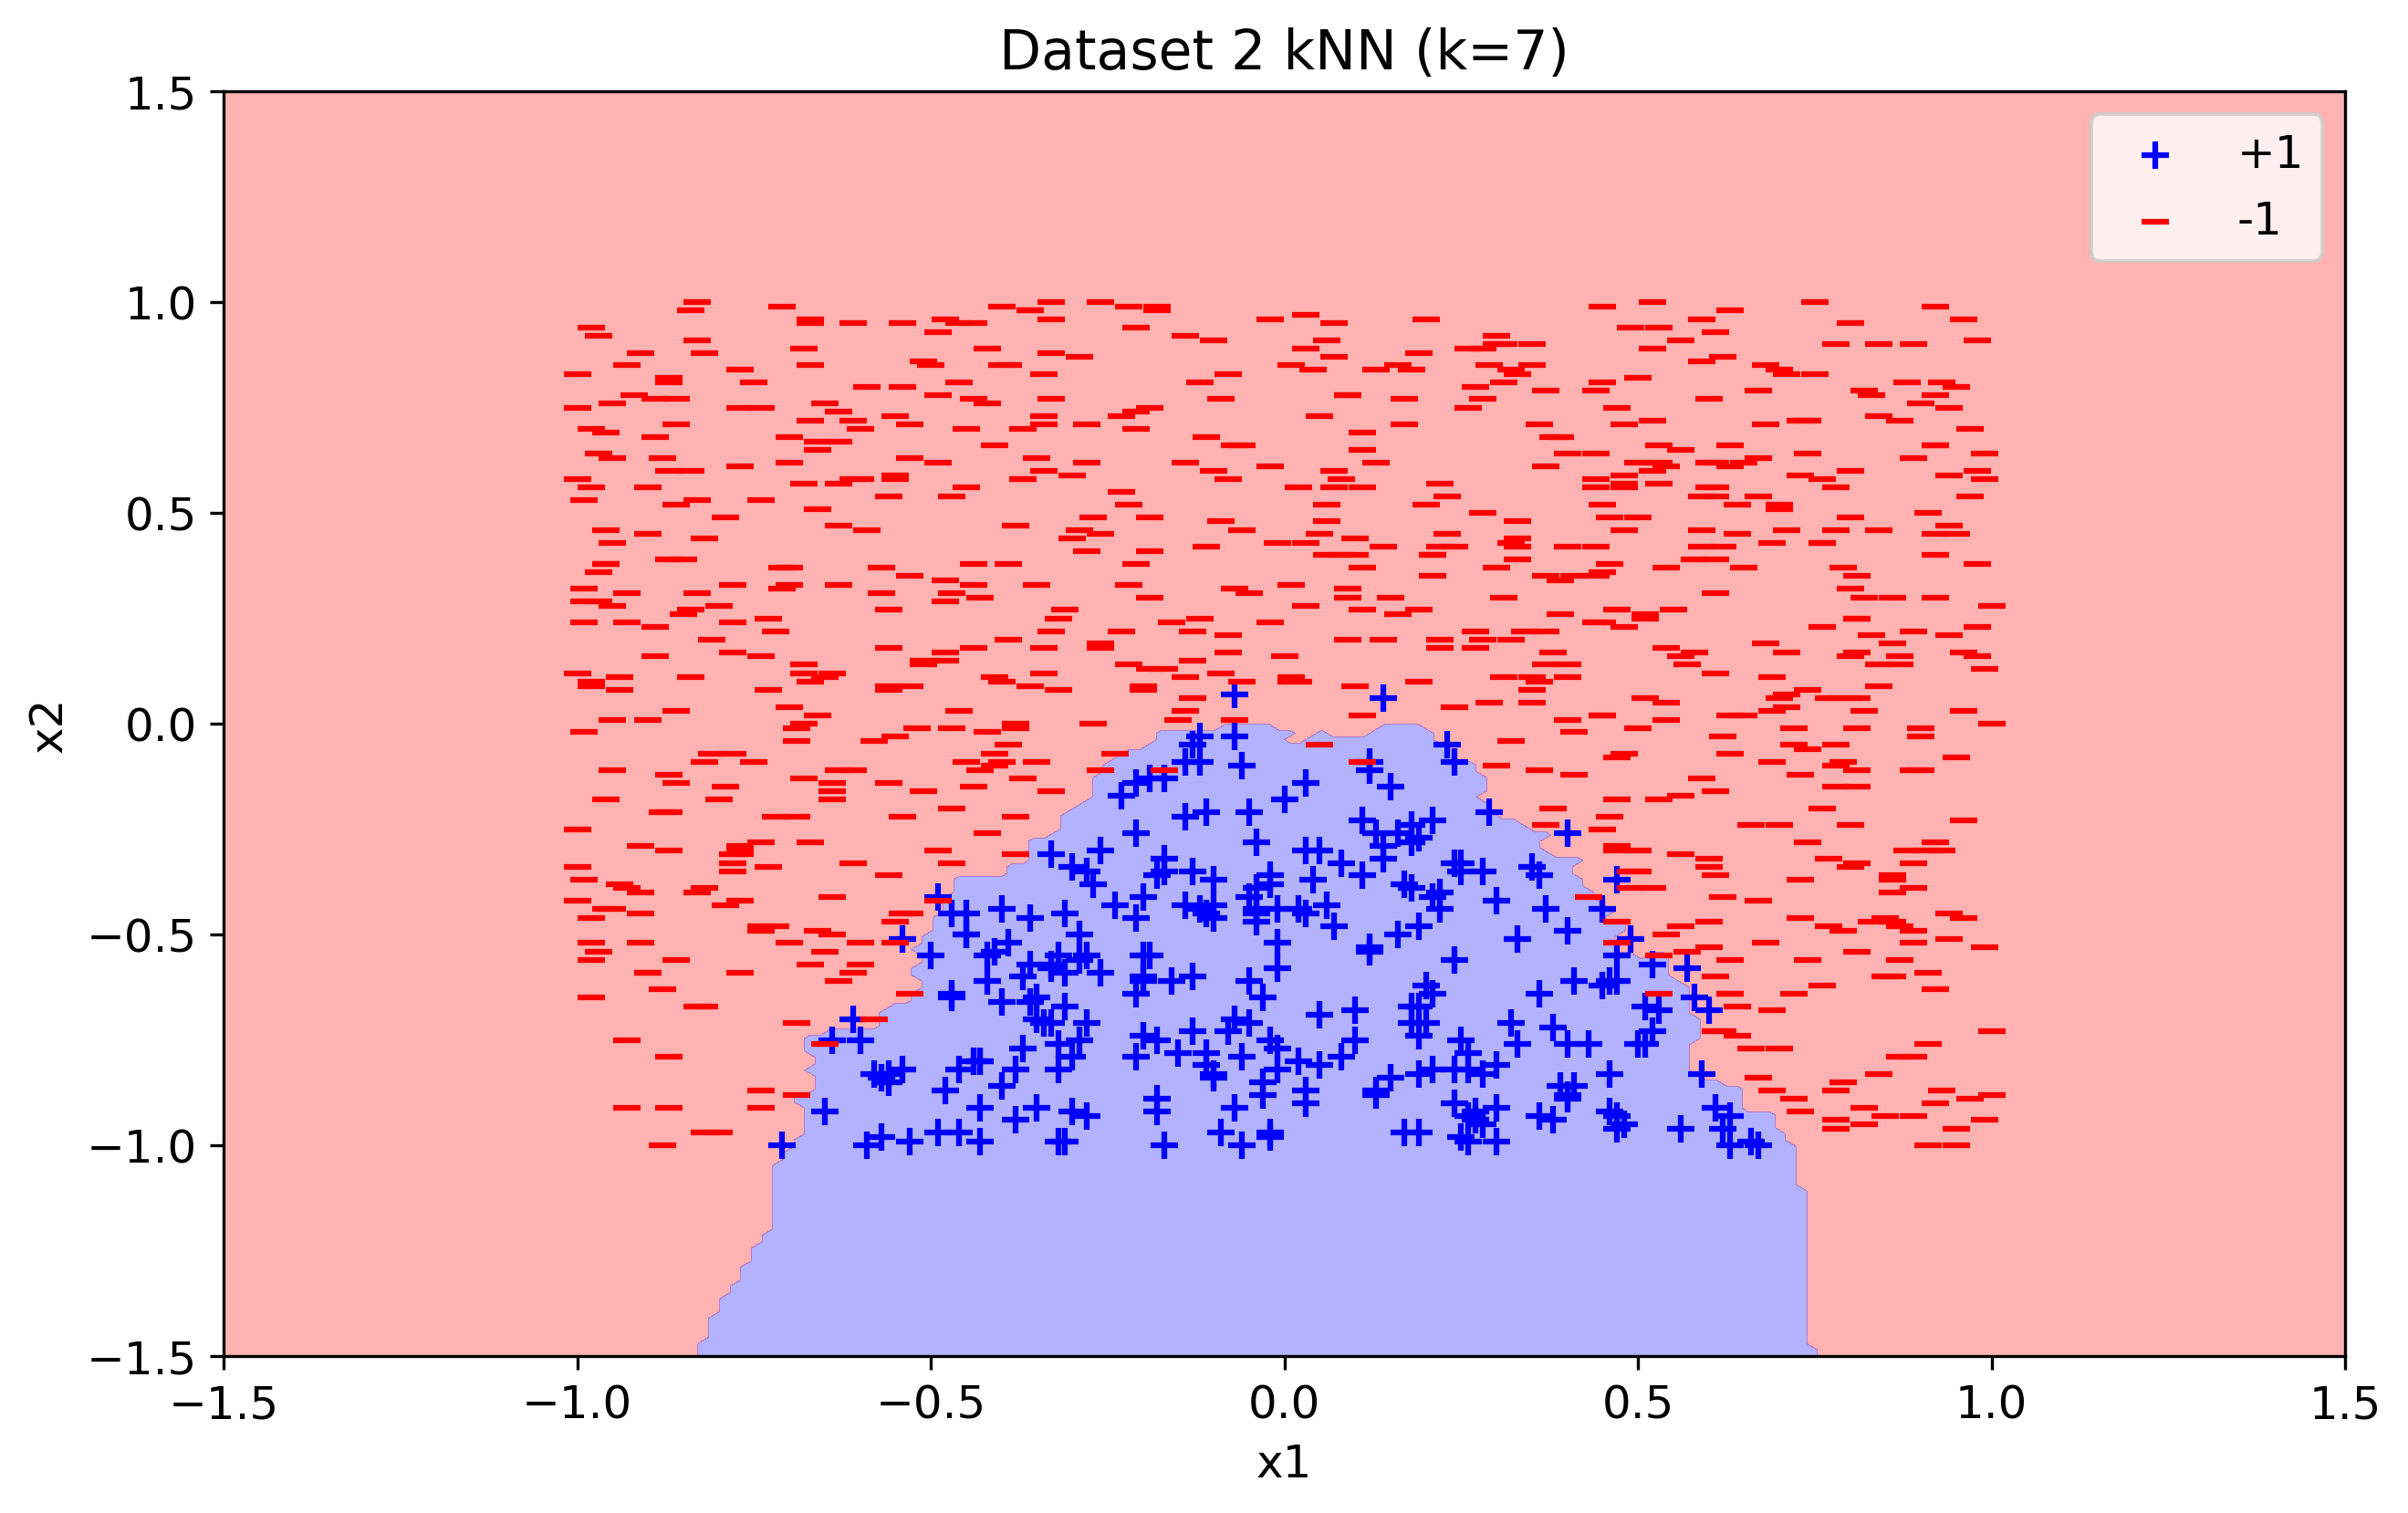
\includegraphics[width=0.5\textwidth]{figures/dataset2_knn_boundary.png}
\caption{Dataset 2 kNN decision boundary with $k=7$.}
\label{fig:dataset2_knn_boundary}
\end{figure}

\subsection*{(c)}

\textbf{Data Source:} Computed on full training data, consistent with Dataset 1 methodology.

\textbf{Logistic Regression ($q=2$, $C=100$):}
\begin{table}[H]
\centering
\begin{tabular}{lcc}
\toprule
 & Predicted -1 & Predicted +1 \\
\midrule
Actual -1 & 794 & 10 \\
Actual +1 & 14 & 261 \\
\bottomrule
\end{tabular}
\end{table}
Metrics: Accuracy=0.9778, TPR=0.9491, FPR=0.0124, Precision=0.9631

\textbf{kNN ($k=7$):}
\begin{table}[H]
\centering
\begin{tabular}{lcc}
\toprule
 & Predicted -1 & Predicted +1 \\
\midrule
Actual -1 & 798 & 6 \\
Actual +1 & 14 & 261 \\
\bottomrule
\end{tabular}
\end{table}
Metrics: Accuracy=0.9815, TPR=0.9491, FPR=0.0075, Precision=0.9775

\textbf{Baseline Most Frequent:}
\begin{table}[H]
\centering
\begin{tabular}{lcc}
\toprule
 & Predicted -1 & Predicted +1 \\
\midrule
Actual -1 & 804 & 0 \\
Actual +1 & 275 & 0 \\
\bottomrule
\end{tabular}
\end{table}
Metrics: Accuracy=0.7451

\textbf{Baseline Random:}
\begin{table}[H]
\centering
\begin{tabular}{lcc}
\toprule
 & Predicted -1 & Predicted +1 \\
\midrule
Actual -1 & 402 & 402 \\
Actual +1 & 139 & 136 \\
\bottomrule
\end{tabular}
\end{table}
Metrics: Accuracy=0.4986

\textbf{Analysis:} Both trained classifiers achieve high accuracy ($>$97\%) with low error rates. Logistic Regression makes 24 total errors; kNN makes 20 errors. Most-frequent baseline achieves 74.51\% accuracy by always predicting the majority class, while random achieves $\sim$50\%.

\subsection*{(d)}

\textbf{Results:}
\begin{itemize}
    \item Logistic Regression: AUC=0.9982
    \item kNN: AUC=0.9977
    \item Most Frequent Baseline: point at (0.0, 0.0)
    \item Random Baseline: point near (0.5, 0.5)
\end{itemize}

\textbf{Observations:} Both ROC curves approach the ideal upper-left corner, indicating near-perfect discrimination. AUC values near 1.0 confirm excellent classifier performance across all operating points. The curves maintain high TPR while keeping FPR minimal, demonstrating robust classification regardless of threshold selection. The most-frequent baseline appears at (0,0) because it predicts all negative for this dataset.

\begin{figure}[H]
\centering
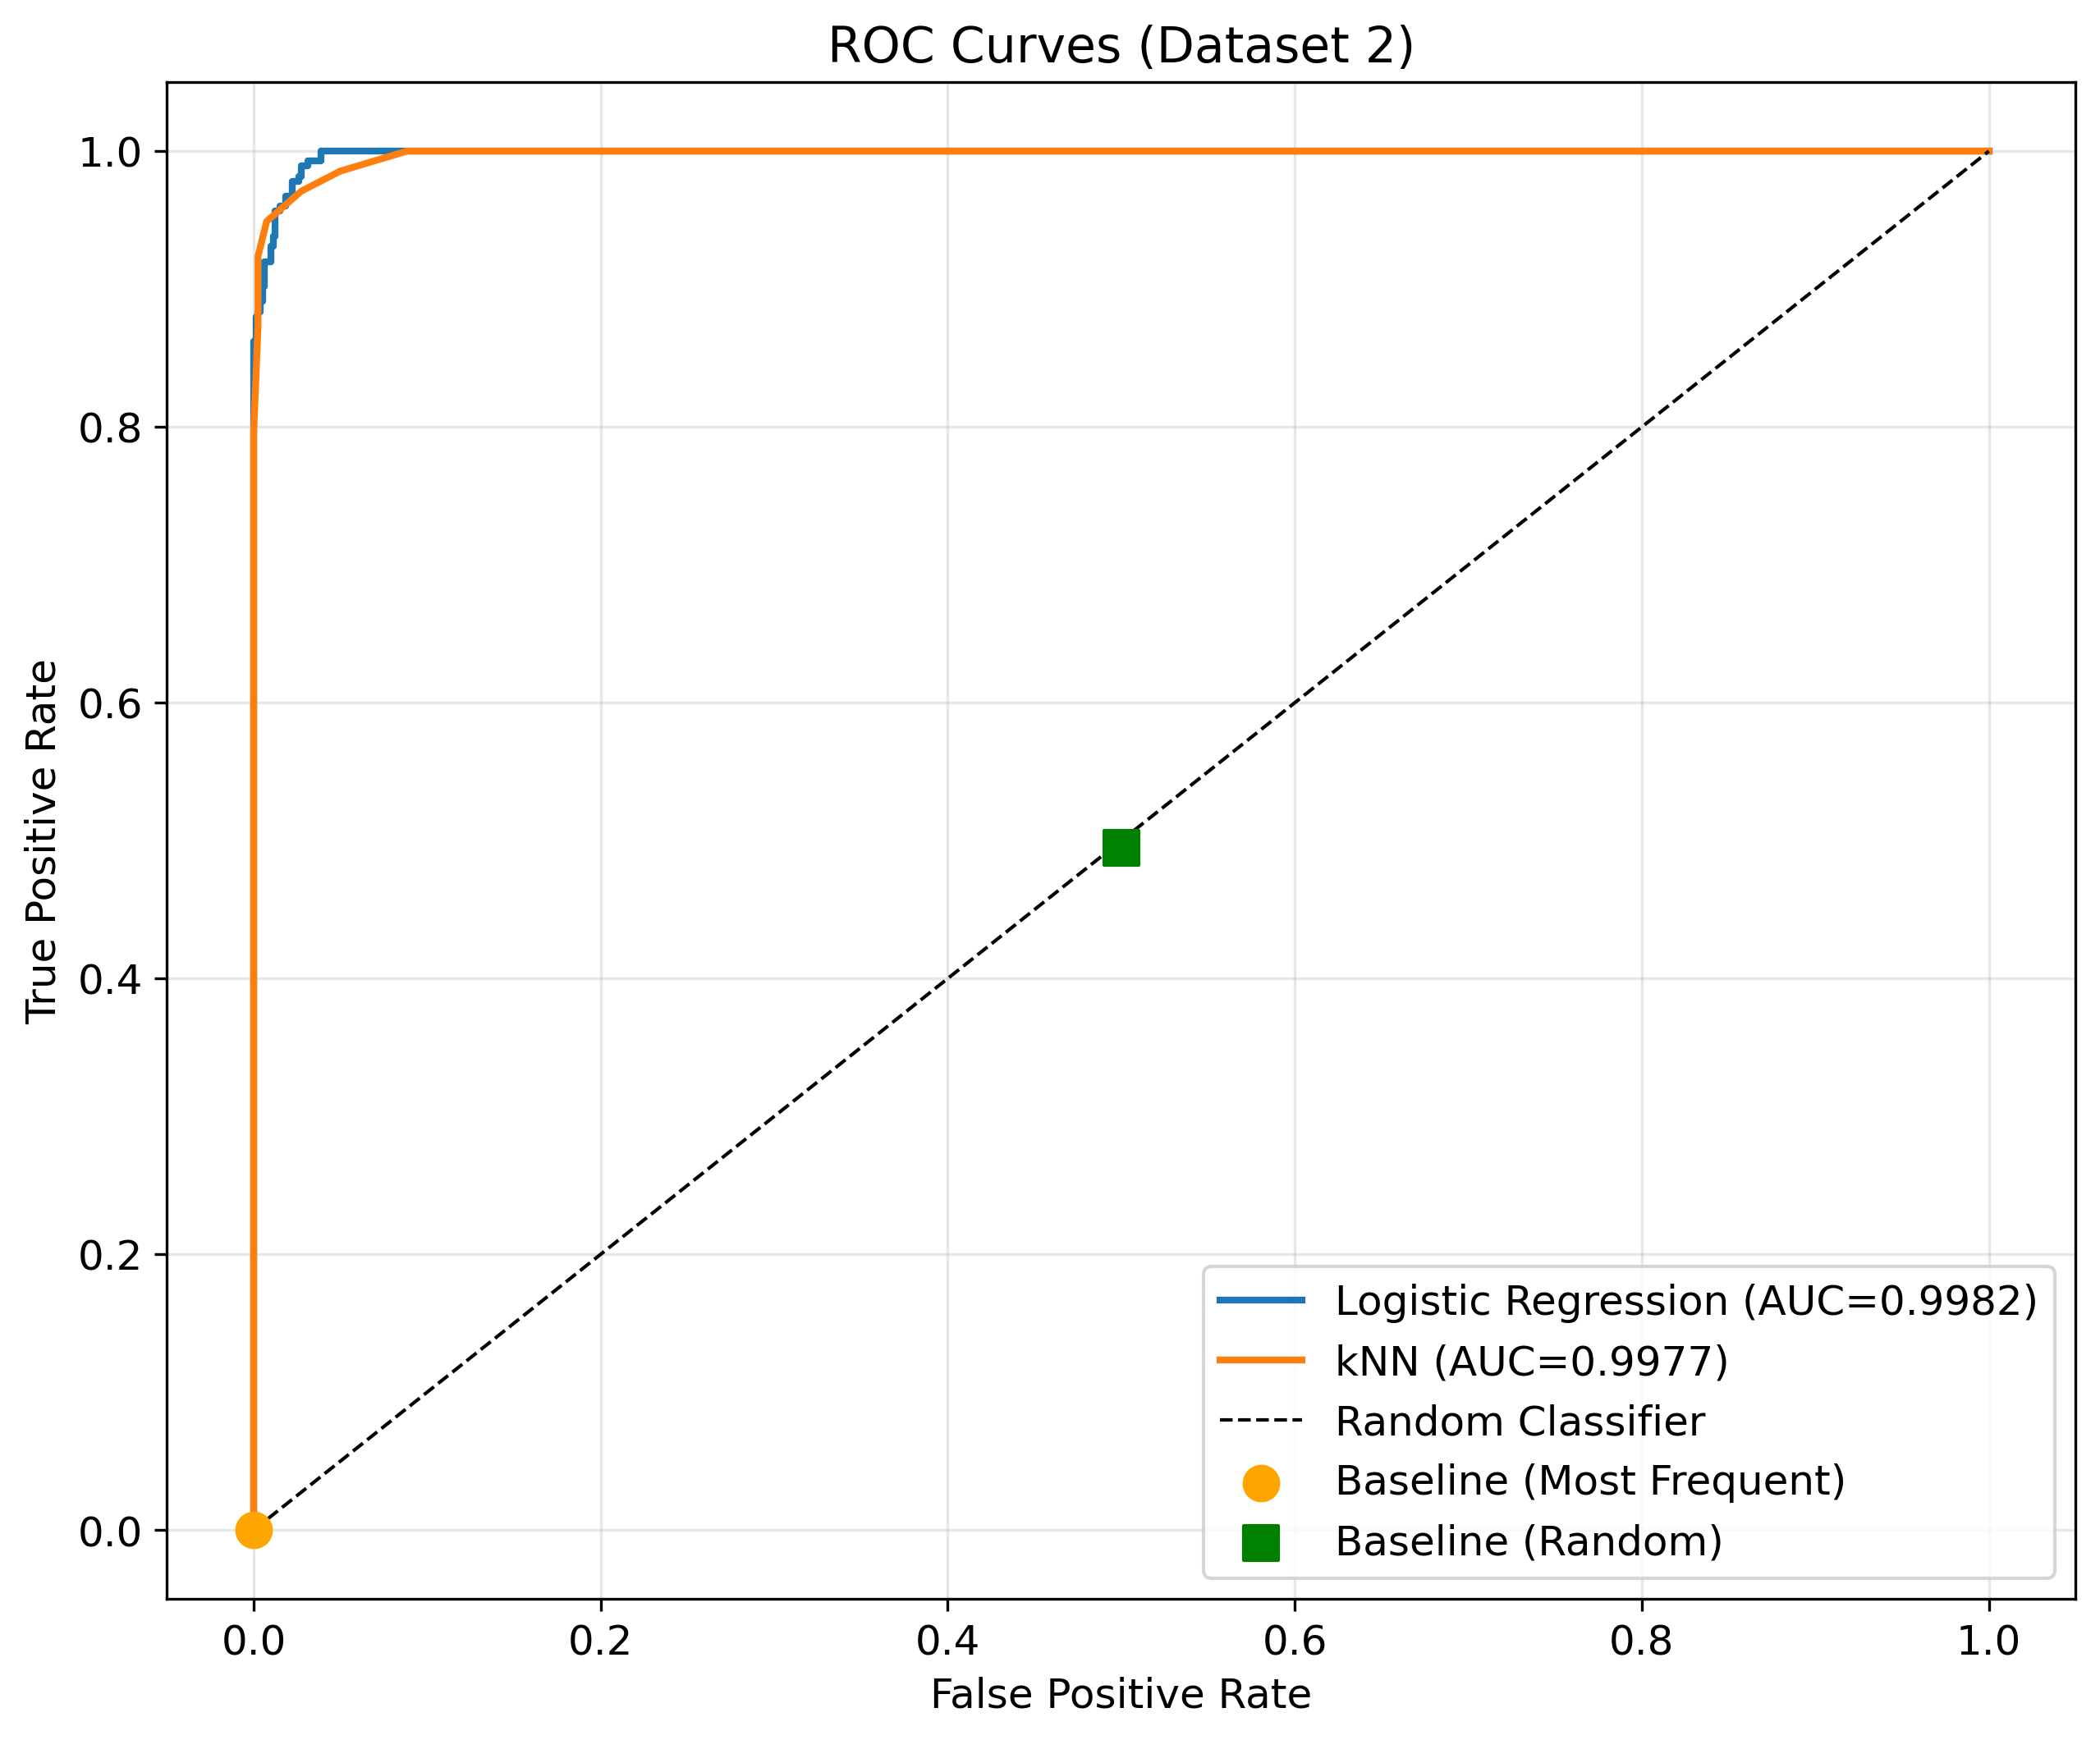
\includegraphics[width=0.5\textwidth]{figures/dataset2_roc.png}
\caption{ROC curves for Dataset 2.}
\label{fig:dataset2_roc}
\end{figure}

\subsection*{(e)}

\textbf{Statistical Performance:} Both classifiers achieve excellent performance with AUC$>$0.99. kNN shows marginally higher accuracy (98.15\% vs 97.78\%) but slightly lower AUC (0.9977 vs 0.9982). These differences are negligible in practical terms.

\textbf{Comparison with Baselines:} Trained classifiers substantially outperform most-frequent baseline by $\sim$24 percentage points (98\% vs 74\%), and random baseline by $\sim$48 percentage points (98\% vs 50\%). This large margin demonstrates genuine learning of discriminative patterns rather than exploitation of class imbalance.

\textbf{ROC Analysis:} The ROC curves' position near (0,1) indicates the classifiers can achieve high sensitivity with minimal false positives. The large separation from the 45° diagonal confirms strong discriminative ability. The dense curve detail reveals stable performance across threshold variations.

\textbf{Classifier Comparison:} Both classifiers perform equivalently well. kNN achieves slightly better accuracy and lower FPR (0.0075 vs 0.0124), while Logistic Regression has marginally higher AUC. Neither difference is statistically or practically significant.

\textbf{Recommendation:}  Either of the classifiers may be used in production. Logistic Re-gression is recommended because: (1) it is interpretable by coefficient inspection, (2) it has faster inference time ($O(n)$ vs $O(nm)$ for kNN), (3) it has smaller deployment footprint (coefficients instead of the entire train
ing set), and (4) easier integration into manufacturing systems. But where high peak accuracy is most important, kNN ($k=7$) is to be preferred.

\textbf{Success Factors:} The classes are well-separated in feature space, with a quadratic boundary sufficient for separation. The characteristics measured accept the discriminative information with less noise, enabling linear and nonlinear models to deliver exceptional results.

\newpage
\section*{APPENDIX}

\begin{lstlisting}
import numpy as np
import matplotlib.pyplot as plt
from sklearn.preprocessing import PolynomialFeatures
from sklearn.linear_model import LogisticRegression
from sklearn.neighbors import KNeighborsClassifier
from sklearn.dummy import DummyClassifier
from sklearn.model_selection import KFold
from sklearn.metrics import confusion_matrix, f1_score, roc_curve, auc

plt.rcParams['figure.figsize'] = (10, 6)
plt.rcParams['font.size'] = 12

# Load and separate datasets
with open('week4.csv', 'r') as f:
    lines = f.readlines()

dataset1_lines = []
dataset2_lines = []
current_dataset = 0

for line in lines:
    if line.startswith('#'):
        current_dataset += 1
        continue
    if current_dataset == 1:
        dataset1_lines.append(line.strip())
    elif current_dataset == 2:
        dataset2_lines.append(line.strip())

data1 = []
for line in dataset1_lines:
    if line:
        data1.append([float(x) for x in line.split(',')])
data1 = np.array(data1)

data2 = []
for line in dataset2_lines:
    if line:
        data2.append([float(x) for x in line.split(',')])
data2 = np.array(data2)

X1 = data1[:, :2]
y1 = data1[:, 2]

X2 = data2[:, :2]
y2 = data2[:, 2]

print('\n' + '='*50)
print('DATASET 1')
print('='*50)
print('Shape:', X1.shape)
print('Class distribution:', np.unique(y1, return_counts=True))

# (i)(a) Logistic Regression with polynomial features
plt.scatter(X1[y1 == -1, 0], X1[y1 == -1, 1], c='blue', label='Class -1', alpha=0.6)
plt.scatter(X1[y1 == 1, 0], X1[y1 == 1, 1], c='red', label='Class +1', alpha=0.6)
plt.xlabel('Feature 1')
plt.ylabel('Feature 2')
plt.title('Dataset 1 Scatter Plot')
plt.legend()
plt.grid(True, alpha=0.3)
plt.savefig('figures/dataset1_scatter.png', dpi=300, bbox_inches='tight')
plt.show()

q_range = [1, 2, 3, 4, 5]
C_range = [0.001, 0.01, 0.1, 1, 10, 100, 1000]
kf = KFold(n_splits=5, shuffle=True, random_state=42)

f1_means = np.zeros((len(q_range), len(C_range)))
f1_stds = np.zeros((len(q_range), len(C_range)))

for i, q in enumerate(q_range):
    poly = PolynomialFeatures(degree=q, include_bias=True)
    X1_poly = poly.fit_transform(X1)
    
    for j, C in enumerate(C_range):
        f1_scores = []
        for train_idx, val_idx in kf.split(X1_poly):
            model = LogisticRegression(C=C, penalty='l2', solver='lbfgs', max_iter=5000)
            model.fit(X1_poly[train_idx], y1[train_idx])
            y_pred = model.predict(X1_poly[val_idx])
            f1_scores.append(f1_score(y1[val_idx], y_pred, pos_label=1))
        
        f1_means[i, j] = np.mean(f1_scores)
        f1_stds[i, j] = np.std(f1_scores)

best_idx = np.unravel_index(np.argmax(f1_means), f1_means.shape)
best_q = q_range[best_idx[0]]
best_C = C_range[best_idx[1]]
best_f1 = f1_means[best_idx]

print(f'\nLogistic Regression: Best q={best_q}, Best C={best_C}, CV F1={best_f1:.4f}')

fig, axes = plt.subplots(1, 2, figsize=(15, 5))

for i, q in enumerate(q_range):
    axes[0].errorbar(C_range, f1_means[i], yerr=f1_stds[i], marker='o', capsize=3, label=f'q={q}')
axes[0].set_xscale('log')
axes[0].set_xlabel('C')
axes[0].set_ylabel('F1 Score')
axes[0].set_title('Dataset 1: Logistic Regression CV (F1 vs C)')
axes[0].legend()
axes[0].grid(True, alpha=0.3)

mean_f1_per_q = np.mean(f1_means, axis=1)
axes[1].bar(q_range, mean_f1_per_q)
axes[1].set_xlabel('Polynomial Degree q')
axes[1].set_ylabel('Mean F1 Score')
axes[1].set_title('Dataset 1: Mean F1 Score by Polynomial Degree')
axes[1].grid(True, alpha=0.3)

plt.tight_layout()
plt.savefig('figures/dataset1_logistic_cv.png', dpi=300, bbox_inches='tight')
plt.show()

poly_best = PolynomialFeatures(degree=best_q, include_bias=True)
X1_poly_best = poly_best.fit_transform(X1)
log_model1 = LogisticRegression(C=best_C, penalty='l2', solver='lbfgs', max_iter=5000)
log_model1.fit(X1_poly_best, y1)

x1_min, x1_max = X1[:, 0].min() - 0.5, X1[:, 0].max() + 0.5
x2_min, x2_max = X1[:, 1].min() - 0.5, X1[:, 1].max() + 0.5
xx1, xx2 = np.meshgrid(np.linspace(x1_min, x1_max, 200), np.linspace(x2_min, x2_max, 200))
X_grid = np.c_[xx1.ravel(), xx2.ravel()]
X_grid_poly = poly_best.transform(X_grid)
Z = log_model1.predict(X_grid_poly).reshape(xx1.shape)

plt.contourf(xx1, xx2, Z, alpha=0.3, levels=[-1.5, 0, 1.5], colors=['blue', 'red'])
plt.scatter(X1[y1 == -1, 0], X1[y1 == -1, 1], c='blue', label='Class -1', edgecolors='k', alpha=0.7)
plt.scatter(X1[y1 == 1, 0], X1[y1 == 1, 1], c='red', label='Class +1', edgecolors='k', alpha=0.7)
plt.xlabel('Feature 1')
plt.ylabel('Feature 2')
plt.title(f'Dataset 1: Logistic Regression Decision Boundary (q={best_q}, C={best_C})')
plt.legend()
plt.grid(True, alpha=0.3)
plt.savefig('figures/dataset1_logistic_boundary.png', dpi=300, bbox_inches='tight')
plt.show()

# (i)(b) kNN Classifier
k_range = [1, 3, 5, 7, 9, 11, 15, 21, 31, 41, 51]
f1_means = []
f1_stds = []

for k in k_range:
    f1_scores = []
    for train_idx, val_idx in kf.split(X1):
        model = KNeighborsClassifier(n_neighbors=k)
        model.fit(X1[train_idx], y1[train_idx])
        y_pred = model.predict(X1[val_idx])
        f1_scores.append(f1_score(y1[val_idx], y_pred, pos_label=1))
    
    f1_means.append(np.mean(f1_scores))
    f1_stds.append(np.std(f1_scores))

best_k_idx = np.argmax(f1_means)
best_k1 = k_range[best_k_idx]

print(f'kNN: Best k={best_k1}, CV F1={f1_means[best_k_idx]:.4f}')

plt.errorbar(k_range, f1_means, yerr=f1_stds, marker='o', capsize=5)
plt.xlabel('k')
plt.ylabel('F1 Score')
plt.title('Dataset 1: kNN Cross-Validation')
plt.grid(True, alpha=0.3)
plt.savefig('figures/dataset1_knn_cv.png', dpi=300, bbox_inches='tight')
plt.show()

knn_model1 = KNeighborsClassifier(n_neighbors=best_k1)
knn_model1.fit(X1, y1)

Z_knn = knn_model1.predict(X_grid).reshape(xx1.shape)

plt.contourf(xx1, xx2, Z_knn, alpha=0.3, levels=[-1.5, 0, 1.5], colors=['blue', 'red'])
plt.scatter(X1[y1 == -1, 0], X1[y1 == -1, 1], c='blue', label='Class -1', edgecolors='k', alpha=0.7)
plt.scatter(X1[y1 == 1, 0], X1[y1 == 1, 1], c='red', label='Class +1', edgecolors='k', alpha=0.7)
plt.xlabel('Feature 1')
plt.ylabel('Feature 2')
plt.title(f'Dataset 1: kNN Decision Boundary (k={best_k1})')
plt.legend()
plt.grid(True, alpha=0.3)
plt.savefig('figures/dataset1_knn_boundary.png', dpi=300, bbox_inches='tight')
plt.show()

# (i)(c) Confusion Matrices
y_pred_log1 = log_model1.predict(X1_poly_best)
y_pred_knn1 = knn_model1.predict(X1)

dummy_freq = DummyClassifier(strategy='most_frequent', random_state=42)
dummy_freq.fit(X1, y1)
y_pred_dummy_freq = dummy_freq.predict(X1)

dummy_uniform = DummyClassifier(strategy='uniform', random_state=42)
dummy_uniform.fit(X1, y1)
y_pred_dummy_uniform = dummy_uniform.predict(X1)

cm_log1 = confusion_matrix(y1, y_pred_log1, labels=[-1, 1])
cm_knn1 = confusion_matrix(y1, y_pred_knn1, labels=[-1, 1])
cm_dummy_freq = confusion_matrix(y1, y_pred_dummy_freq, labels=[-1, 1])
cm_dummy_uniform = confusion_matrix(y1, y_pred_dummy_uniform, labels=[-1, 1])

print('\nConfusion Matrices:')
print(f'Logistic Regression - Accuracy: {(cm_log1[0,0] + cm_log1[1,1]) / cm_log1.sum():.4f}')
print(f'kNN - Accuracy: {(cm_knn1[0,0] + cm_knn1[1,1]) / cm_knn1.sum():.4f}')
print(f'Baseline (Most Frequent) - Accuracy: {(cm_dummy_freq[0,0] + cm_dummy_freq[1,1]) / cm_dummy_freq.sum():.4f}')
print(f'Baseline (Random) - Accuracy: {(cm_dummy_uniform[0,0] + cm_dummy_uniform[1,1]) / cm_dummy_uniform.sum():.4f}')

# (i)(d) ROC Curves
y_scores_log1 = log_model1.decision_function(X1_poly_best)
y_scores_knn1 = knn_model1.predict_proba(X1)[:, 1]

fpr_log1, tpr_log1, _ = roc_curve(y1, y_scores_log1, pos_label=1)
fpr_knn1, tpr_knn1, _ = roc_curve(y1, y_scores_knn1, pos_label=1)

auc_log1 = auc(fpr_log1, tpr_log1)
auc_knn1 = auc(fpr_knn1, tpr_knn1)

plt.figure(figsize=(8, 8))
plt.plot(fpr_log1, tpr_log1, label=f'Logistic Regression (AUC={auc_log1:.4f})', linewidth=2)
plt.plot(fpr_knn1, tpr_knn1, label=f'kNN (AUC={auc_knn1:.4f})', linewidth=2)
plt.plot([0, 1], [0, 1], 'k--', label='Random Classifier', linewidth=1)

tpr_freq = cm_dummy_freq[1,1] / (cm_dummy_freq[1,0] + cm_dummy_freq[1,1])
fpr_freq = cm_dummy_freq[0,1] / (cm_dummy_freq[0,0] + cm_dummy_freq[0,1])
plt.plot(fpr_freq, tpr_freq, 'ro', markersize=10, label='Most Frequent Baseline')

tpr_uniform = cm_dummy_uniform[1,1] / (cm_dummy_uniform[1,0] + cm_dummy_uniform[1,1])
fpr_uniform = cm_dummy_uniform[0,1] / (cm_dummy_uniform[0,0] + cm_dummy_uniform[0,1])
plt.plot(fpr_uniform, tpr_uniform, 'gs', markersize=10, label='Random Baseline')

plt.xlabel('False Positive Rate')
plt.ylabel('True Positive Rate')
plt.title('Dataset 1: ROC Curves')
plt.legend(loc='lower right')
plt.grid(True, alpha=0.3)
plt.savefig('figures/dataset1_roc.png', dpi=300, bbox_inches='tight')
plt.show()

print(f'\nAUC: Logistic Regression={auc_log1:.4f}, kNN={auc_knn1:.4f}')

# ==================== DATASET 2 ====================

print('\n' + '='*50)
print('DATASET 2')
print('='*50)
print('Shape:', X2.shape)
print('Class distribution:', np.unique(y2, return_counts=True))

# (ii)(a) Logistic Regression with polynomial features
plt.scatter(X2[y2 == -1, 0], X2[y2 == -1, 1], c='blue', label='Class -1', alpha=0.6)
plt.scatter(X2[y2 == 1, 0], X2[y2 == 1, 1], c='red', label='Class +1', alpha=0.6)
plt.xlabel('Feature 1')
plt.ylabel('Feature 2')
plt.title('Dataset 2 Scatter Plot')
plt.legend()
plt.grid(True, alpha=0.3)
plt.savefig('figures/dataset2_scatter.png', dpi=300, bbox_inches='tight')
plt.show()

f1_means = np.zeros((len(q_range), len(C_range)))
f1_stds = np.zeros((len(q_range), len(C_range)))

for i, q in enumerate(q_range):
    poly = PolynomialFeatures(degree=q, include_bias=True)
    X2_poly = poly.fit_transform(X2)
    
    for j, C in enumerate(C_range):
        f1_scores = []
        for train_idx, val_idx in kf.split(X2_poly):
            model = LogisticRegression(C=C, penalty='l2', solver='lbfgs', max_iter=5000)
            model.fit(X2_poly[train_idx], y2[train_idx])
            y_pred = model.predict(X2_poly[val_idx])
            f1_scores.append(f1_score(y2[val_idx], y_pred, pos_label=1))
        
        f1_means[i, j] = np.mean(f1_scores)
        f1_stds[i, j] = np.std(f1_scores)

best_idx = np.unravel_index(np.argmax(f1_means), f1_means.shape)
best_q = q_range[best_idx[0]]
best_C = C_range[best_idx[1]]
best_f1 = f1_means[best_idx]

print(f'\nLogistic Regression: Best q={best_q}, Best C={best_C}, CV F1={best_f1:.4f}')

fig, axes = plt.subplots(1, 2, figsize=(15, 5))

for i, q in enumerate(q_range):
    axes[0].errorbar(C_range, f1_means[i], yerr=f1_stds[i], marker='o', capsize=3, label=f'q={q}')
axes[0].set_xscale('log')
axes[0].set_xlabel('C')
axes[0].set_ylabel('F1 Score')
axes[0].set_title('Dataset 2: Logistic Regression CV (F1 vs C)')
axes[0].legend()
axes[0].grid(True, alpha=0.3)

mean_f1_per_q = np.mean(f1_means, axis=1)
axes[1].bar(q_range, mean_f1_per_q)
axes[1].set_xlabel('Polynomial Degree q')
axes[1].set_ylabel('Mean F1 Score')
axes[1].set_title('Dataset 2: Mean F1 Score by Polynomial Degree')
axes[1].grid(True, alpha=0.3)

plt.tight_layout()
plt.savefig('figures/dataset2_logistic_cv.png', dpi=300, bbox_inches='tight')
plt.show()

poly_best = PolynomialFeatures(degree=best_q, include_bias=True)
X2_poly_best = poly_best.fit_transform(X2)
log_model2 = LogisticRegression(C=best_C, penalty='l2', solver='lbfgs', max_iter=5000)
log_model2.fit(X2_poly_best, y2)

x1_min, x1_max = X2[:, 0].min() - 0.5, X2[:, 0].max() + 0.5
x2_min, x2_max = X2[:, 1].min() - 0.5, X2[:, 1].max() + 0.5
xx1, xx2 = np.meshgrid(np.linspace(x1_min, x1_max, 200), np.linspace(x2_min, x2_max, 200))
X_grid = np.c_[xx1.ravel(), xx2.ravel()]
X_grid_poly = poly_best.transform(X_grid)
Z = log_model2.predict(X_grid_poly).reshape(xx1.shape)

plt.contourf(xx1, xx2, Z, alpha=0.3, levels=[-1.5, 0, 1.5], colors=['blue', 'red'])
plt.scatter(X2[y2 == -1, 0], X2[y2 == -1, 1], c='blue', label='Class -1', edgecolors='k', alpha=0.7)
plt.scatter(X2[y2 == 1, 0], X2[y2 == 1, 1], c='red', label='Class +1', edgecolors='k', alpha=0.7)
plt.xlabel('Feature 1')
plt.ylabel('Feature 2')
plt.title(f'Dataset 2: Logistic Regression Decision Boundary (q={best_q}, C={best_C})')
plt.legend()
plt.grid(True, alpha=0.3)
plt.savefig('figures/dataset2_logistic_boundary.png', dpi=300, bbox_inches='tight')
plt.show()

# (ii)(b) kNN Classifier
f1_means = []
f1_stds = []

for k in k_range:
    f1_scores = []
    for train_idx, val_idx in kf.split(X2):
        model = KNeighborsClassifier(n_neighbors=k)
        model.fit(X2[train_idx], y2[train_idx])
        y_pred = model.predict(X2[val_idx])
        f1_scores.append(f1_score(y2[val_idx], y_pred, pos_label=1))
    
    f1_means.append(np.mean(f1_scores))
    f1_stds.append(np.std(f1_scores))

best_k_idx = np.argmax(f1_means)
best_k2 = k_range[best_k_idx]

print(f'kNN: Best k={best_k2}, CV F1={f1_means[best_k_idx]:.4f}')

plt.errorbar(k_range, f1_means, yerr=f1_stds, marker='o', capsize=5)
plt.xlabel('k')
plt.ylabel('F1 Score')
plt.title('Dataset 2: kNN Cross-Validation')
plt.grid(True, alpha=0.3)
plt.savefig('figures/dataset2_knn_cv.png', dpi=300, bbox_inches='tight')
plt.show()

knn_model2 = KNeighborsClassifier(n_neighbors=best_k2)
knn_model2.fit(X2, y2)

Z_knn = knn_model2.predict(X_grid).reshape(xx1.shape)

plt.contourf(xx1, xx2, Z_knn, alpha=0.3, levels=[-1.5, 0, 1.5], colors=['blue', 'red'])
plt.scatter(X2[y2 == -1, 0], X2[y2 == -1, 1], c='blue', label='Class -1', edgecolors='k', alpha=0.7)
plt.scatter(X2[y2 == 1, 0], X2[y2 == 1, 1], c='red', label='Class +1', edgecolors='k', alpha=0.7)
plt.xlabel('Feature 1')
plt.ylabel('Feature 2')
plt.title(f'Dataset 2: kNN Decision Boundary (k={best_k2})')
plt.legend()
plt.grid(True, alpha=0.3)
plt.savefig('figures/dataset2_knn_boundary.png', dpi=300, bbox_inches='tight')
plt.show()

# (ii)(c) Confusion Matrices
y_pred_log2 = log_model2.predict(X2_poly_best)
y_pred_knn2 = knn_model2.predict(X2)

dummy_freq2 = DummyClassifier(strategy='most_frequent', random_state=42)
dummy_freq2.fit(X2, y2)
y_pred_dummy_freq2 = dummy_freq2.predict(X2)

dummy_uniform2 = DummyClassifier(strategy='uniform', random_state=42)
dummy_uniform2.fit(X2, y2)
y_pred_dummy_uniform2 = dummy_uniform2.predict(X2)

cm_log2 = confusion_matrix(y2, y_pred_log2, labels=[-1, 1])
cm_knn2 = confusion_matrix(y2, y_pred_knn2, labels=[-1, 1])
cm_dummy_freq2 = confusion_matrix(y2, y_pred_dummy_freq2, labels=[-1, 1])
cm_dummy_uniform2 = confusion_matrix(y2, y_pred_dummy_uniform2, labels=[-1, 1])

print('\nConfusion Matrices:')
print(f'Logistic Regression - Accuracy: {(cm_log2[0,0] + cm_log2[1,1]) / cm_log2.sum():.4f}')
print(f'kNN - Accuracy: {(cm_knn2[0,0] + cm_knn2[1,1]) / cm_knn2.sum():.4f}')
print(f'Baseline (Most Frequent) - Accuracy: {(cm_dummy_freq2[0,0] + cm_dummy_freq2[1,1]) / cm_dummy_freq2.sum():.4f}')
print(f'Baseline (Random) - Accuracy: {(cm_dummy_uniform2[0,0] + cm_dummy_uniform2[1,1]) / cm_dummy_uniform2.sum():.4f}')

# (ii)(d) ROC Curves
y_scores_log2 = log_model2.decision_function(X2_poly_best)
y_scores_knn2 = knn_model2.predict_proba(X2)[:, 1]

fpr_log2, tpr_log2, _ = roc_curve(y2, y_scores_log2, pos_label=1)
fpr_knn2, tpr_knn2, _ = roc_curve(y2, y_scores_knn2, pos_label=1)

auc_log2 = auc(fpr_log2, tpr_log2)
auc_knn2 = auc(fpr_knn2, tpr_knn2)

plt.figure(figsize=(8, 8))
plt.plot(fpr_log2, tpr_log2, label=f'Logistic Regression (AUC={auc_log2:.4f})', linewidth=2)
plt.plot(fpr_knn2, tpr_knn2, label=f'kNN (AUC={auc_knn2:.4f})', linewidth=2)
plt.plot([0, 1], [0, 1], 'k--', label='Random Classifier', linewidth=1)

tpr_freq = cm_dummy_freq2[1,1] / (cm_dummy_freq2[1,0] + cm_dummy_freq2[1,1])
fpr_freq = cm_dummy_freq2[0,1] / (cm_dummy_freq2[0,0] + cm_dummy_freq2[0,1])
plt.plot(fpr_freq, tpr_freq, 'ro', markersize=10, label='Most Frequent Baseline')

tpr_uniform = cm_dummy_uniform2[1,1] / (cm_dummy_uniform2[1,0] + cm_dummy_uniform2[1,1])
fpr_uniform = cm_dummy_uniform2[0,1] / (cm_dummy_uniform2[0,0] + cm_dummy_uniform2[0,1])
plt.plot(fpr_uniform, tpr_uniform, 'gs', markersize=10, label='Random Baseline')

plt.xlabel('False Positive Rate')
plt.ylabel('True Positive Rate')
plt.title('Dataset 2: ROC Curves')
plt.legend(loc='lower right')
plt.grid(True, alpha=0.3)
plt.savefig('figures/dataset2_roc.png', dpi=300, bbox_inches='tight')
plt.show()

print(f'\nAUC: Logistic Regression={auc_log2:.4f}, kNN={auc_knn2:.4f}')
\end{lstlisting}

\end{document}

